%TODO
%extract every sectoin to files, 'cause it's hard to handle such big file
%add points in main page title
%change font size in Рисунок 1
%add count item to Рисунок 1, should be section and them count number
%chnage - for --- where needed
%check for goog wrapping
%check for borders and font size and 1.5 space (print document there and in office)
%chek printing exuality as is in PDF http://forum.ixbt.com/topic.cgi?id=23:27770
%add italic to subsubsection
% TODO - fix caption centering in all tables

%%% initial
\documentclass[ukrainian,14pt,utf8,
%pointsection, % це хз для чого
nocolumnsxix,
nocolumnxxxi,
nocolumnxxxii,
floatsection, %підпис плаваючих об'єктів згдіно номера розліду (таблиці, рисунки)
hpadding=5mm, %відстань до рамки зліва, справа
vpadding=5mm %відстань до рамки зліва, справа
]{eskdtext}

%%% for working with math
%\usepackage{amsmath}
%\usepackage{amssymb}

%%% for working some LaTeX packages
\usepackage{xecyr}

%%% for fonts
\usepackage{xltxtra}
%%% Times New Roman - main font
\setmainfont[Mapping=tex-text]{Times New Roman}
%%% Courier New - fot math
\setmonofont[Scale=MatchLowercase]{Courier New}

%%% for ---, --, << >> и т.п.
\defaultfontfeatures{Mapping=tex-text}

%%% ukrainian text
\usepackage{polyglossia}
\setdefaultlanguage{ukrainian}
\newfontfamily\ukrainianfont{Times New Roman}

%%% for words wrapping
%\XeTeXinterchartokenstate=1
%\XeTeXcharclass `\- 24
%\XeTeXinterchartoks 24 0 ={\hskip\z@skip}
%\XeTeXinterchartoks 0 24 ={\nobreak}

% для абзацу %
\usepackage{indentfirst}

% code highlighting %
\usepackage{listings}
\lstset{
language=Java,
basicstyle=\footnotesize\sffamily,
numbers=left,
numberstyle=\tiny,
frame=tb,
columns=fullflexible,
showstringspaces=false,
breaklines=true 
}

% automaticaly wrap to other line
\sloppy
%\usepackage{setspace}
%\onehalfspacing
\linespread{1.5}

%%% for graphix
\usepackage{graphicx}
\graphicspath{{images/}} %path to images
%%% titile for pictures
\addto{\captionsukrainian}{\renewcommand{\figurename}{Рисунок}}


%%% for internet ulrs
\usepackage{url}

%%% subtitiles(\subsubsection) don't show in article
%\setcounter{tocdepth}{2}

%%% new section from new page
\let\stdsection\section
\renewcommand\section{\newpage\stdsection}

%%% плаваючі обєкти підпис
%\renewcommand\section{\newpage\stdsection}

%%% Numering subtopics begin with B (B.1)
%\makeatletter
%\renewcommand\thesubsection{\ifnum\c@section=0{В.\arabic{subsection}}\else{\arabic{section}.\arabic{subsection}}\fi}
%\makeatother

%%% for coloring rows
\usepackage[table]{xcolor}

%%% для розриву таблиць 
\usepackage{longtable}
%\usepackage{eskdgraph}






\ESKDtitle{ Аналіз розробки програмного алгоритмічного забезпечення багатофункціональної корпоративної системи для сумісної роботи, управління документами і проектами }
\ESKDdocName{\uppercase{Звіт з переддипломної практики}}
\ESKDgroup{ІНФТУНГ ПЗ-07-1}

\ESKDauthor{ Бойчук Я.В. }
\ESKDchecker{ Бандура В.В. }
\ESKDsignature{ ПП.ПЗ 03.00.00.000 ПЗ }

%%finixg ukrainian languale%%
\renewcommand{\ESKDcolumnXfIname}{Розробив}
\renewcommand{\ESKDcolumnXfIIname}{Перевірив}
\renewcommand{\ESKDcolumnXfIVname}{Т.контр}
\renewcommand{\ESKDcolumnXfVname}{Н.контр}
\renewcommand{\ESKDcolumnXfVIname}{Затв.}

\renewcommand{\ESKDcolumnIVname}{Літ.}
\renewcommand{\ESKDcolumnVIIIname}{Аркушів}
\renewcommand{\ESKDcolumnXVIIname}{Підпис}
\renewcommand{\ESKDcolumnXVname}{Арк.}

%%fix ESKDTitle font
%%FIXME change for row, now for font
\renewcommand{\ESKDfontVsize}{%
\ESKDfontSetBaseLineStretch
\fontsize{10pt}{8pt}\selectfont\ESKDfontShape}

%%space after text
\setlength{\ESKDsectionSkipBefore}{-7mm \@plus -3mm \@minus -2mm}
\setlength{\ESKDsectionSkipAfter}{7mm \@plus 1mm \@minus 2mm}
\setlength{\ESKDsubsectionSkipBefore}{-7mm \@plus -3mm \@minus -2mm}
\setlength{\ESKDsubsectionSkipAfter}{7mm \@plus 1mm \@minus 2mm}
\setlength{\ESKDsubsubsectionSkipBefore}{-7mm \@plus -3mm \@minus -2mm}
\setlength{\ESKDsubsubsectionSkipAfter}{7mm \@plus 1mm \@minus 2mm}

%%font size for section (&&sub)
\renewcommand{\ESKDsectionStyle}{\centering\normalfont\bfseries\MakeUppercase}
\renewcommand{\ESKDsubsectionStyle}{\centering\normalfont\bfseries}
\renewcommand{\ESKDsubsubsectionStyle}{\centering\normalfont\bfseries}




        


\begin{document}
%і\fontsize{14}{14pt}\selectfont

%\maketitle


\setcounter{page}{6}
\tableofcontents

%\section*{Вступ}
%\addcontentsline{toc}{section}{Вступ}
%Текст вступу
%

\section*{ПЕРЕЛІК УМОВНИХ СКОРОЧЕНЬ}
\addcontentsline{toc}{section}{ПЕРЕЛІК УМОВНИХ СКОРОЧЕНЬ}
\par СКБД -- Система керування базою даних
\par API -- Application programming interface
\par JPA -- Java Persistence API
\par SQL -- Structured Query Language
\par GUI -- Graphical User Interface
\par UML -- Unified Modelling Language
\par MCC(MVCC) -- Multiversion concurrency control


\section*{ВСТУП}
\addcontentsline{toc}{section}{ВСТУП}
В нас час важливою економічною точкою опори для будь-якої комерційної організації є наявність певних факторів, які визнають чітку позицію компанії на ринку. До всіх цих чинників можна віднести багато варіантів, зокрема:
\begin{itemize}
\item капітал підприємства;
\item матеріальна база;
\item технічна база;
\item кваліфікований персонал;
\item місце підприємства на внутрішньому і зовнішньому ринку;
\item наявність сучасних засобів виробництва та ведення бізнесу;
\item та інші.
\end{itemize}

Тому кожний розділ ведення бізнесу повинний бути детально розглянутий та впроваджений у життя. 
Але якщо подивитися із точки зору програмного забезпечення, то на даному етапі розвитку цивілізації, якісне ПЗ відіграє напевно найбільш важливу роль. 
Адже не можливо зараз утримувати всі дані в паперовому вигляді, не можливо відсилати друковані листи, чи спілкуватися тільки по телефоні і взнавати новини компанії тільки при зустрічі. 
У наш стрімкий час розвитку, новини міняються із колосальною швидкістю, тому встигнути за всім просто не можливо без певного програмного продукту. 
Уявіть собі інформатор, який сповіщає будь-які для Вас новини чи корисну інформацію в зручний для Вас час, при цьому вміє фільтрувати і аналізувати дані із попередніх запитів. 
Також на даний момент важко уявити не можливість спільної роботи над документами, над електронними таблицями. 
Дані технології вже давно використовуються людьми і підприємствами, починаючи від найменших де працює двоє людей, до величезних із кількістю працівників більше ста тисяч. 
Але для цього всього використовуються дуже багато технологій, які важко налаштувати і потребують великих витрат на підтримку.
Тому було розроблено багато сервісів і додатків, які полегшують роботу в мережі для підприємств.
\par Дане ПЗ використовується у всіх нішах нашого життя, починаючи від шкіл і лікарень, закінчуючи величезними корпораціями з будівництва космічних кораблів. 
Тому розробити універсальний продукт, який забезпечить всі вимоги, просто не можливо. 
Для кожної сфери існують свої нюанси.
\par Цікавою нішею для дослідження стало корпоративне програмне забезпечення для малого і середнього бізнесу.
 На даний момент існує багато програмних продуктів для комерційних цілей, проте вони здебільшого розраховані на великі корпорації і підприємства.
Тому використання їх для менших фірм просто не доцільно, або дуже складно із фінансової сторони (витрати на підтримку передують вигоді).
Як відомо, на ринку до цих пір зберігається тенденція на попит на корпоративне програмне забезпечення, яке б відповідало вимогам малого і середнього бізнесу, і в той же час було практично придатним для використання у великих корпоративних цілях


\section{АНАЛІЗ РИНКУ І ПОТОЧНИХ РІШЕНЬ}
На даний момент існує досить багато готових рішень корпоративних порталів. 
Вони можуть забезпечувати підприємства всіма необхідними функціями і додатками, починаючи від системи обліку працівників, і завершуючи системою аналітики та збору даних -- все це залежить від потреб ринку і певної компанії.
Проте майже всі вони здебільшого призначені для великих компаній, і невеличкі компанії або повинні витрачати величезні гроші на купівлю ліцензій, або ж не користуватися усіма перевагами корпоративного порталу.
Тому було проведено загальний огляд продуктів і виділено основні переваги і недоліки, також виділено поточну використовувану ліценцію розповсюдження ПЗ.
\subsection{Переваги та недоліки поточних рішень}
Зробивши аналіз даної сфери, можна виділити декілька основних аспектів, які будуть використані для розробки подальшого програмного продукту.
Левова частка програмного забезпечення корпоративних порталів розроблено згідно стандартів\cite{portlet2}. 
Всі додатки і аплікації можуть без проблем взаємодіяти між собою. 
Проте великою їх нестачею для малої сфери бізнесу є закритість програмного коду і величезна вартість ліцензій.
Тому невеличкі компанії (до 100 людей) просто не мають змоги собі дозволити таку <<розкіш>>.

\subsubsection{Ліцензіювання і відкритість АРІ}
\par Було проведено аналіз поточних продуктів і їх ліцензій, і виявлено, що майже 90\% використовує проприєтарні рішення.
Більш детально розглянуто у таблиці \ref{t:portals}:

{\footnotesize
\begin{longtable}{|c|c|c|}
\captionsetup{justification=centering}
\caption{Список корпоративних порталів і використовувана ліцензія}\label{t:portals}\\
\hline
\multicolumn{1}{|c|}{\textbf{Назва продукту}}&
\multicolumn{1}{c|}{\textbf{Технологія}}&
\multicolumn{1}{c|}{\textbf{Ліцензія}}\\\hline

\endfirsthead
\caption*{\hfill Продовження таблиці \ref{t:portals}}\\\hline

\multicolumn{1}{|c|}{\textbf{Назва продукту}}&
\multicolumn{1}{c|}{\textbf{Технологія}}&
\multicolumn{1}{c|}{\textbf{Ліцензія}}\\\hline
\endhead

 Jetspeed & Java EE & Apache License v2.0\\ \hline
 ATG Portal & Java EE & Proprietary\\ \hline
 Backbase Portal Software & Java EE, .NET & Proprietary \\ \hline 
 Broadvision Portal & Java EE & Proprietary \\ \hline 
 Bluenog ICE & Java EE & Proprietary \\ \hline
 enPortal  & Java EE & Proprietary\\ \hline 
 CommunityManager.NET  & .NET & Proprietary \\ \hline
 eXo Portal & Java EE & Affero General Public License \\ \hline
 eXo Platform & Java EE & Proprietary \\ \hline
 GateIn Portal & Java EE & LGPL \\ \hline
 Hippo CMS & Java EE & Open Source and Proprietary Licenses \\ \hline
 WebSphere Portal & Java EE & Proprietary \\ \hline
 TeamPortal & Java EE & Proprietary \\ \hline
 JBoss Enterprise Portal  & Java EE & LGPL \\ \hline
 IntraNet & ASP.NET & Proprietary \\ \hline
 Liferay Portal & Java EE & Proprietary Licenses \\ \hline
 TeamWox Groupware & C++ & Proprietary \\ \hline
 SharePoint Server & ASP.NET & Proprietary \\ \hline
 Vignette Portal 8.0 & Java EE & Proprietary \\ \hline
 Oracle WebCenter Suite 11g & Java EE & Proprietary \\ \hline
 Oracle WebLogic Portal 10g & Java EE & Proprietary \\ \hline
 Oracle WebCenter Interaction 10g & ASP.NET & Proprietary \\ \hline
 Oracle IAS Portal 10g & Java EE & Proprietary \\ \hline
 Regroup & Ruby & Proprietary \\ \hline
 ACUBE Portal 5.0 & Java EE & Proprietary \\ \hline
 SAP NetWeaver 7.0 & Java EE & Proprietary \\ \hline
 SORCE V9 & ASP.NET & Proprietary \\ \hline
 Sun Java System Portal Server & Java EE & Open Source, licensing \& support plans \\ \hline
 Sun GlassFish Web Space Server  & Java EE & Open Source, licensing \& support plans \\ \hline
 tmsEKP 1.52 & Java EE & Proprietary \\ \hline
 PortalBuilder 5.2 & Java EE & Proprietary \\ \hline
 ProPortal 4.0 & Java EE & Proprietary \\ \hline
 Intrexx & Java EE & Proprietary \\ \hline
 uPortal & Java EE & Apache License v2.0 \\ \hline

\end{longtable}
}


\par Зробивши певний аналіз, можна дійти до висновку, якби невеликим компаніям давати можливість використовувати продукт на підставах вільного розповсюдження коду, то вони б охотніше пробували, і з часом інвестували в нього гроші, або ж просто <<купляли>> підтримку.
Тобто використати одну із відкритих ліцензій типу GNU Public License.
\par Економічна вигода продукту буде базуватися на корпоративній платній підтримці, типу все, починаючи від підбору серверів -- до налаштування і підтримки продукту.
Зате розробники будуть мати змогу додавати свої зміни у загальний репозиторій та виправляти помилки, що значною мірою пришвидшить процес розробки.
Основна стратегія розробки буде націлена на швидкий вихід на ринок і пошук потенційних клієнтів.
Також велика увага буде прикута до ринку пострадянських республік, адже на даний момент ринок бізнесу стрімко розвивається, тобто попит є, а пропозиція не повній мірі відповідає потребі.
Портали, які розробляються, переважно націлені на Європейський та Американський ринок, а також Азію.
Тому, базуючись на цьому, було виділено такі основні вимоги, як врахування нашого законодавства (для прикладу по працевлаштуванню працівників, веденню документації, конвертації валют і тому подібне) та локалізацію сервісу.
Тим більше підтримка користувачів буде набагато легша і ефективніша всередині країни, ніж з-за кордону, що дасть нам перевагу над іншими існуючими продуктами.

\par Також велику увагу буде приділено відкритості АРІ для взаємодії із вже існуючими додатками.
Адже існуючі рішення в основному базуються на закритих протоколах, чим саме змушують користувачів прив'язуватися до їхньої системи і залежати від них.
\par Інтерфейс і система всіх сучасних продуктів дуже <<важкі>> і мульти-функціональні, що потребує затрат значних ресурсів як у користувачів так і на стороні сервера.
Цей аспект також буде максимально спрощений, що в свою чергу дозволить продукту виділитися на ринку малого бізнесу.

\subsection{Технології розробки} 
Базуючись на поточних стандартах \cite{portlet2} та використовуваних базових технологій (таблиця \ref{t:portals}) було прийнято рішення впровадити розробку на базі Java.
Адже саме Sun (зараз Oracle) <<диктує>> моду на ринку стандартизації портлетів, тому буде просто пристосуватися до поточних рішень.
\par Звичайно ж буде використано всі переваги Java EE.
Для гнучкої і швидкої розробки буде застосовано Spring Framework із ORM обгорткою Hibernate поверх бази даних MySQL.
Для фронтенд логіки UI в основному буде використовуватися jQuery фреймворк.
Сервер бекенду буде працювати на Apache Tomcat.
\par На даний момент не планується стандартизація щодо портлетів, просто в майбутньому можливо буде виділено цей пункт для реалізації в системі.

\subsubsection{Мова програмування Java}
\par Java (вимовляється Джава; інколи - Ява) -- об'єктно-орієнтована мова програмування, випущена компанією Sun Microsystems у 1995 році як основний компонент платформи Java. Синтаксис мови багато в чому походить від C та C++. У офіційній реалізації, Java програми компілюються у байткод, який при виконанні інтерпретується віртуальною машиною для конкретної платформи.
\par Sun Microsystems (Oracle) надає компілятор Java та віртуальну машину Java, які задовольняють специфікації Java Community Process, під ліцезією GNU General Public License.
\par Мова значно запозичила синтаксис із C і C++. Зокрема, взято за основу об'єктну модель С++, проте її модифіковано. Усунуто можливість появи деяких конфліктних ситуацій, що могли виникнути через помилки програміста та полегшено сам процес розробки об'єктно-орієнтованих програм. Ряд дій, які в С/C++ повинні здійснювати програмісти, доручено віртуальній машині. Передусім, Java розроблялась як платформо-незалежна мова, тому вона має менше низькорівневих можливостей для роботи з апаратним забезпеченням. За необхідності таких дій java дозволяє викликати підпрограми, написані іншими мовами програмування.

\par Мова програмування Java зародилася в 1991 р. в лабораторіях компанії Sun Microsystems. Розробку проекту започаткував Джеймс Ґослінґ, сам проект мав назву <<Green>>(Зелений). Створення першої робочої версії, яка мала назву <<Oak>>(дуб), зайняло 18 місяців. Оскільки виявилось, що ім'я Oak уже використовувалось іншою фірмою, то в результаті тривалих суперечок навколо назви нової мови з поміж ряду запропонованих було вибрано назву Java, у 1995 р. мову було офіційно перейменовано.
\par Головним мотивом створення Java була потреба в мові програмування, яка б не залежала від платформи (тобто від архітектури) і яку можна було б використовувати для створення програмного забезпечення, яке вбудовується в різноманітні побутові електронні прилади, такі як мобільні засоби зв'язку, пристрої дистанційного керування тощо.
\par Досить скоро майже всі найпопулярніші тогочасні веб-оглядачі отримали можливість запускати <<безпечні>> для системи Java аплети всередині веб-сторінок. У грудні 1998 р. Sun Microsystems випустила Java 2 (спершу під назвою J2SE 1.2), де було реалізовано декілька конфігурацій для різних типів платформ. Наприклад, J2EE призначалася для створення корпоративних застосунків, а значно урізана J2ME для приладів з обмеженими ресурсами, таких як мобільні телефони. У 2006 році в маркетингових цілях, Версії J2 було перейменовано у Java EE, Java ME та Java SE, відповідно.
\par 13 листопада 2006 року Sun випустили більшу частину Java в якості вільного та відкритого програмного забезпечення згідно з умовами GNU General Public License (GPL). 8 травня 2007 корпорація закінчила процес, в результаті якого всі початкові коди Java були випущенні під GPL, за винятком невеликої частини коду, на який Sun не мала авторського права.
\par Період становлення Java збігся у часі з розквітом міжнародної інформаційної служби World Wide Web. Ця обставина відіграла вирішальну роль у майбутньому Java, оскільки Web теж вимагала платформо-незалежних програм. Як наслідок, були зміщені акценти в розробці Sun з побутової електроніки на програмування для Інтернет.

\par Під <<незалежністю від архітектури>> мається на увазі те, що програма, написана на мові Java, працюватиме на будь-якій підтримуваній апаратній чи системній платформі без змін у початковому коді та перекомпіляції.
\par Цього можна досягти, компілюючи початковий Java код у байт-код, який являє собою спрощені машинні команди. Потім програму можна виконати на будь-якій платформі, що має встановлену віртуальну машину Java, яка інтерпретує байткод у код, пристосований до специфіки конкретної операційної системи і процесора. Зараз віртуальні машини Java існують для більшості процесорів і операційних систем.
\par Стандартні бібліотеки забезпечують загальний спосіб доступу до таких платформозалежних особливостей, як обробка графіки, багатопотоковість та роботу з мережами. У деяких версіях задля збільшення продуктивності JVM, байт-код можна компілювати у машинний код до або під час виконання програми.
\par Основна перевага використання байт-коду -- це портативність. Тим не менш, додаткові витрати на інтерпретацію означають, що інтерпретовані програми будуть майже завжди працювати повільніше, ніж скомпільовані у машинний код, і саме тому Java одержала репутацію <<повільної>> мови. Проте, цей розрив суттєво скоротився після введення декількох методів оптимізації у сучасних реалізаціях JVM.
\par Одним із таких методів є англ. just-in-time (JIT) компіляція, що перетворює Java байт-код у машинний під час першого запуску програми, а потім кешує його. У результаті, така програма запускається і виконується швидше, ніж простий інтерпретований код, але ціною додаткових витрат на компіляцію під час виконання. Складніші віртуальні машини також використовують динамічну рекомпіляцію, яка полягає в тому, що віртуальна машина аналізує поведінку запущеної програми й вибірково рекомпілює та оптимізує певні її частини. З використанням динамічної рекомпіляції можна досягти більшого рівня оптимізації, ніж за статичної компіляції, оскільки динамічний компілятор може робити оптимізації на базі знань про довкілля періоду виконання та про завантажені класи. До того ж, він може виявляти так звані гарячі точки (англ. hot spots) -- частини програми, найчастіше внутрішні цикли, які займають найбільше часу при виконанні. JIT компіляція та динамічна рекомпіляція збільшує швидкість Java програм, не втрачаючи при цьому портативності.
\par Існує ще одна технологія оптимізації байткоду, широко відома як статична компіляція, або англ. ahead-of-time (AOT) компіляція. Цей метод передбачає, як і традиційні компілятори, безпосередню компіляцію у машинний код. Це забезпечує хороші показники в порівнянні з інтерпретацією, але за рахунок втрати переносності: скомпільовану таким способом програму можна запустити тільки на одній, цільовій платформі.
\par Швидкість офіційної віртуальної машини Java значно покращилася з моменту випуску ранніх версій, до того ж, деякі випробування показали, що продуктивність JIT компіляторів у порівнянні зі звичайними компіляторами у машинний код майже однакова. Проте ефективність компіляторів не завжди свідчить про швидкість виконання скомпільованого коду, тільки ретельне тестування може виявити справжню ефективність у даній системі.

\par На противагу C++, Java <<об'єктно-орієнтованіша>>. Всі дані і дії групуються в класи об'єктів. Виключенням з повної об'єктності (як скажімо в Smalltalk) є примітивні типи (int, float тощо). Це було свідомим рішенням проектувальників мови задля збільшення швидкості. Через це, Java не вважається повністю об'єктно-орієнтовною мовою.
\par У Java всі об'єкти є похідними від головного об'єкта (він називається просто Object), з якого вони успадковують базову поведінку і властивості.
\par Хоча у C++ вперше стало доступне множинне успадкування, але у Java можливе тільки одинарне успадкування, завдяки чому виключається можливість конфліктів між членами класу(методи і змінні), які успадковуються від базових класів.

\par Java використовує автоматичний збирач сміття для керування пам'яттю під час життєвого циклу об'єкта. Програміст вирішує, коли створювати об'єкти, а віртуальна машина відповідальна за звільнення пам'яті після того, як об'єкт стає непотрібним. Коли до певного об'єкта вже не залишається посилань, збирач сміття може автоматично прибирати його із пам'яті. Проте, витік пам'яті все ж може статися, якщо код, написаний програмістом, має посилання на вже непотрібні об'єкти, наприклад на об'єкти, що зберігаються у діючих контейнерах.
\par Прибирання сміття дозволене у будь-який час. В ідеалі воно відбувається під час бездіяльності програми. Збірка сміття автоматично форсується при нестачі вільної пам'яті в купі для розміщення нового об'єкта, що може призводити до кількасекундного зависання. Тому існують реалізації віртуальної машини Java з прибиральником сміття спеціально створеним для програмування систем реального часу.

\subsubsection{Огляд Java Enterprise Edition, як системи розробки бізнес рішень}
\par Java Platform Enterprise Edition, скорочено Java EE (до версії 5.0 — Java 2 Enterprise Edition або J2EE) -- набір специфікацій і відповідної документації для мови Java, який описує архітектуру серверної платформи для задач середніх і великих підприємств.
\par Специфікації деталізовані настільки, щоб забезпечити переносимість програм з однієї реалізації платформи на іншу. Основна мета специфікацій -- забезпечити масштабованість програми і цілісність даних під час роботи системи. Java EE орієнтована на використання її через веб як в Інтернеті, так і в локальних мережах. Вся специфікація створюється і затверджується через JCP (Java Community Process) в рамках ініціативи Sun Microsystems Inc (тепер Oracle).
\par Java EE є промисловою технологією і в основному використовується в високопродуктивних проектах, в яких є необхідна надійність, масштабованість, гнучкість.
\par Популярності Java EE також сприяє те, що Sun (Oracle) пропонує безкоштовний комплект розробки, SDK, який дозволяє підприємствам розробляти свої системи, не витрачаючи великих коштів. В цей комплект входить сервер програм з ліцензією для розробки.

\subsubsection{Об'єктно-реляційне відображення}
\par ORM (англ. Object-relational mapping, Обє'ктно-реляційна проекція) -- технологія програмування, яка зв'язує бази даних з концепціями об'єктно-орієнтованих мов програмування, створюючи <<віртуальну об'єктну базу даних>>.
\par У об'єктно-орієнтованому програмуванні об'єкти в програмі представляють об'єкти з реального світу. Як приклад можна розглянути адресну книгу, яка містить список людей разом з кількома телефонами і кількома адресами. В термінах об'єктно-орієнтованого програмування вони представлятимуться об'єктами класу <<Людина>>, які міститимуть наступний список полів: ім'я, список (або масив) телефонів і список адрес.
\par Суть проблеми полягає в перетворенні таких об'єктів у форму, в якій вони можуть бути збережені у файлах або базах даних, і які легко можуть бути витягнуті в подальшому, зі збереженням властивостей об'єктів і відносин між ними. Ці об'єкти називають <<постійними>> (англ. persistent). Історично існує кілька підходів до рішення цієї задачі.

\par Вирішення проблеми зберігання даних існує -- це реляційні системи управління базами даних. Використання реляційної бази даних для зберігання об'єктно-орієнтованих даних приводить до семантичного провалу, примушуючи програмістів писати програмне забезпечення, яке повинне уміти як обробляти дані в об'єктно-орієнтованому вигляді, так і вміти зберегти ці дані в реляційній формі. Ця постійна необхідність в перетворенні між двома різними формами даних не тільки сильно знижує продуктивність, але і створює труднощі для програмістів, оскільки обидві форми даних накладають обмеження одна на одну.
\par Реляційні бази даних використовують набір таблиць, що представляють прості дані. Додаткова або зв'язана інформація зберігається в інших таблицях. Часто для зберігання одного об'єкта в реляційній базі даних використовується декілька таблиць -- це, у свою чергу, вимагає застосування операції JOIN для отримання всієї інформації, що відноситься до об'єкта, для її обробки. Наприклад, в розглянутому варіанті із записною книгою, для зберігання даних, швидше за все, використовуватимуться як мінімум дві таблиці: <<люди>> і <<адреси>>, і, можливо, навіть таблиця з телефонними номерами.
\par Оскільки системи управління реляційними базами даних зазвичай не реалізують реляційного представлення фізичного рівня зв'язків, виконання кількох послідовних запитів (що відносяться до однієї <<об'єктно-орієнтованої>> структури даних) може бути дуже витратне. Зокрема, один запит вигляду <<знайти такого-то користувача і всі його телефони і всі його адреси і повернути їх у такому форматі>> швидше за все, буде виконаний швидше за серію запитів вигляду <<Знайти користувача. Знайти його адреси. Знайти його телефони>>. Це відбувається завдяки роботі оптимізатора і витратам на синтаксичний аналіз запиту.
\par Деякі реалізації ORM автоматично синхронізують завантажені в пам'ять об'єкти з базою даних. Для того, щоб це було можливим, після створення SQL-запиту, що перетворює об'єкт в SQL, отримані дані копіюються в поля об'єкта, як у всіх інших реалізаціях ORM. Після цього об'єкт повинен стежити за змінами цих значень і записувати їх у базу даних.
\par Системи управління реляційними базами даних показують хорошу продуктивність на глобальних запитах, які зачіпають велику ділянку бази даних, але об'єктно-орієнтований доступ ефективніший при роботі з малими об'ємами даних, оскільки це дозволяє скоротити семантичний провал між об'єктною і реляційною формами даних.
При одночасному існуванні цих двох різних світів збільшується складність об'єктного коду для роботи з реляційними базами даних, і він стає схильнішим до помилок. Розробники програмного забезпечення, що ґрунтується на базах даних, шукали легший спосіб досягнення постійності їхніх об'єктів.
\par Розроблено безліч пакетів, що знімають необхідність в перетворенні об'єктів для зберігання в реляційних базах даних.
Деякі пакети вирішують цю проблему, надаючи бібліотеки класів, здатних виконувати такі перетворення автоматично. Маючи список таблиць в базі даних і об'єктів в програмі, вони автоматично перетворять запити з одного вигляду в іншій. В результаті запиту об'єкта <<людина>> (з прикладу з адресною книгою) необхідний SQL-запит буде сформований і виконаний, а результати <<магічним>> чином перетворені в об'єкти <<номер телефону>> всередині програми.
\par З погляду програміста система повинна виглядати як постійне сховище об'єктів. Він може просто створювати об'єкти і працювати з ними як завжди, а вони автоматично зберігатимуться в реляційній базі даних.
\par На практиці все не так просто і очевидно. Всі системи ORM зазвичай проявляють себе в тому або іншому вигляді, зменшуючи в деякому роді можливість ігнорування бази даних. Більш того, шар транзакцій може бути повільним і неефективним (особливо в термінах згенерованого SQL). Все це може привести до того, що програми працюватимуть повільніше і використовувати більше пам'яті, чим програми, написані <<вручну>>.
\par Але ORM позбавляє програміста від написання великої кількості коду, часто одноманітного і схильного до помилок, тим самим значно підвищуючи швидкість розробки. Крім того, більшість сучасних реалізацій ORM дозволяють програмістові при необхідності жорстко задати код SQL-запитів, який використовуватиметься при тих або інших діях (збереження в базу даних, завантаження, пошук тощо) з постійним об'єктом.

\subsubsection{jQeury, як система для розробки UI}
\par jQuery -- популярна JavaScript-бібліотека з відкритим програмним кодом. Вона була представлена у січні 2006 року у BarCamp NYC Джоном Ресіґом (John Resig). Використовується більш ніж 31\% від 10,000 найбільш відвідуваних сайтів. jQuery є найпопулярнішою бібліотекою JavaScript, яка потужно використовується на сьогоднішній день\cite{jquery_usage}.
\par jQuery є вільним відкритим програмним забезпеченням з подвійним ліцензуванням під MIT License та GNU General Public License другої версії. Синтаксис jQuery розроблений, щоб зробити орієнтування у навігації зручнішим завдяки вибору елементів DOM, створенню анімації, обробки подій, і розробки AJAX-застосувань. jQuery також надає можливості для розробників, для створення плагінів у верхній частині бібліотеки JavaScript. Використовуючи ці об'єкти, розробники можуть створювати абстракції для низькорівневої взаємодії та створювати анімацію для ефектів високого рівня. Це сприяє створенню потужних і динамічних веб-сторінок.
\par Основне завдання jQuery -- це надавати розробнику легкий та гнучкий інструментарій кросбраузерної адресації DOM об'єктів за допомогою CSS та XPath селекторів. Також даний фреймворк надає інтерфейси для AJAX-застосувань, обробників подій і простої анімації.
Принцип роботи jQuery полягає в використанні класу (функції), який при звертанні до нього повертає сам себе. Таким чином, це дозволяє будувати послідовний ланцюг методів.
\par Бібліотека jQuery є JavaScript файлом, яка включає всю його DOM, події(events), ефекти(effects), і AJAX функції. Вона може бути додана до web-сторінки посиланням на локальну копію, або на одну з копій доступних на публічному сервері (наприклад Google CDN).


\subsubsection{Apache Tomcat -- фронтенд сервер розробки}
\par Apache Tomcat -- контейнер сервлетів, розроблений Apache Software Foundation. Повністю написаний мовою програмування Java та реалізує специфікацію сервлетів і Java Server Pages від Sun Microsystems (Oracle), що є стандартами для розробки веб-застосунків на Java.
\par Члени ASF і незалежні добровольці розвивають та підтримують Tomcat. Користувачі мають вільний доступ до вихідного коду Tomcat за умовами Apache License. Першою релізною версією Tomcat стала версія 3.0.x (попередні версії були випущені Sun для внутрішнього користування).



\subsection{Технічний огляд продукту}
Розглянемо більш детально пункт про наявність сучасних засобів ведення бізнесу. 
Кожна компанія завжди стикається із проблемою ведення обліку працівників, ведення обліку фінансів, спільної роботи над документами та іншим.
Також є величезна і невід'ємна потреба у спільному доступі до документів, до корпоративного календаря, до блогу користувачів, до електронних таблиць та інформаційної дошки.
\par Портал підприємства (також відомий як enterprise information portal (EIP) або корпоративний портал) є основою для інтеграції інформації, людей і процесів в рамках організації. 
Це дає змогу забезпечити єдину точку доступу, часто у вигляді веб-інтерфейсу і призначеної для агрегування та персоналізації інформації за допомогою конкретних програмних додатків. Однією відмінною рисою корпоративних порталів є децентралізоване внесення контенту, управління і збереження на віддаленому сервері та постійне оновлення.


\subsection{Історичний огляд корпоративної сфери}
В середині 1990-х років появилися такі веб-портали як AltaVista, AOL, Excite і Yahoo. 
Вони забезпечували користувачів певним набором функцій (наприклад новини, електронна пошта, погода, котирування акцій і пошук), які часто були представлені у вигляді автономного порталу.
Незабаром підприємства усіх типів і форм почали бачити необхідність аналогічного функціоналу для їх різноманітних потреб, проте із єдиною точкою доступу.
\par До кінця 1990-х років, виробники програмного забезпечення почали розробляти веб-портали для різних підприємств. 
Ці програмні пакети були розроблені таким чином, щоб підприємства могли легко розгортати свої власні налаштування корпоративного порталу та доповнювати його своїми додатками.
Перші постачальники комерційних веб порталів з'явилися в 1998 році, це були такі фірми як: Epicentric, Plumtree  та Viador. 
Ці фірми були основними гравцями на ринку, проте ситуація змінилася в 2002 року, коли на ринок почали виходити постачальники серверних аплікацій, такі як BEA, IBM, Passageways, Oracle Corporation і Sun Microsystems.
Підприємства могли вибрати для своїх цілей декілька порталів, що базувалося на основі їх бізнес-структури та стратегічної спрямованості.
\par У 2003 році розробники Java-порталів випустили стандарт, відомий як JSR-168. 
Він повинен був визначити API для взаємодії між корпоративними порталами та портлетами.
Постачальники програмного забезпечення почали розробляти JSR-168 сумісні портлети, які можуть бути розгорнуті на будь-якому JSR-168 сумісному корпоративному порталі. 
Другий ітераційний стандарт JSR-286 є остаточним на даний момент і випущений 12 червня 2008 року.

\subsection{Портлети}
Портлет -- це змінний компонент інтерфейсу веб-порталу (елемент веб--сторінки), який можливо певним чином підключити до порталу.
Портлет містить в собі фрагменти розмітки, які вбудовуються в сторінку порталу. 
Найчастіше сторінка порталу представляється у вигляді набору портлетів, які взаємодіють між собою. 
Таким чином, портлет (або сукупність портлетів) представляється у вигляді єдиного веб-додатку, розміщеного на порталі. 
Приклади портлетів можуть бути наступними: електронна пошта, повідомлення про погоду, фінансовий стан, останні новини і тому подібне.
Завдяки існуючим стандартам розробники можуть створювати портлети, що легко вбудовуються в будь-який портал, який слідує стандартам і правилам.
\par Існує протокол WSRP, що забезпечує стандарт веб-сервісів і дозволяє автоматично вбудовувати віддалено запущені портлети з різних джерел.
Специфікація Java-портлетів JSR168 дає можливість взаємодіяти між собою портлетам з різних веб-порталів. 
Ця специфікація визначає безліч API для взаємодії контейнерів портлетів і дає різні адреси областей персоналізації, подання та безпеки.
Існує безліч постачальників комерційних контейнерів портлетів. 
Як відомо лідирують у цій галузі IBM, Oracle, Vignette. 
Реалізації від цих постачальників мають додаткові розширення і налаштування, проте деякі із ним можуть бути не затверджені стандартами. 
Крім того, є портали з відкритим вихідним кодом, що підтримують JSR168, такі як корпоративний портал Apache Jetspeed-2 або eXo Portal.
\subsubsection{Apache Pluto}
Розглянемо на прикладі один з найбільш вдалої реалізації стандарту портлетів JSR168 -- це Apache Pluto.
Портлет працює всередині контейнера портлетів (Pluto).
Цей контейнер містить портлет з необхідним середовищем для подальшого виконання.
Контейнер портлетів керує життєвим циклом всіх вікон порталу та надає інтерфейси для портлетів, котрі викликаються всередині нього.
Контейнер також запускає методи на виконання із доступних цільових користувацьких сторінок і взаємодіє із сторінками порталу. Принцип роботи і архітектурні компоненти аплікації Pluto 2.0. зображено на рисунку \ref{pic:pluto}.

    \begin{figure}[!ht]
		\centering
		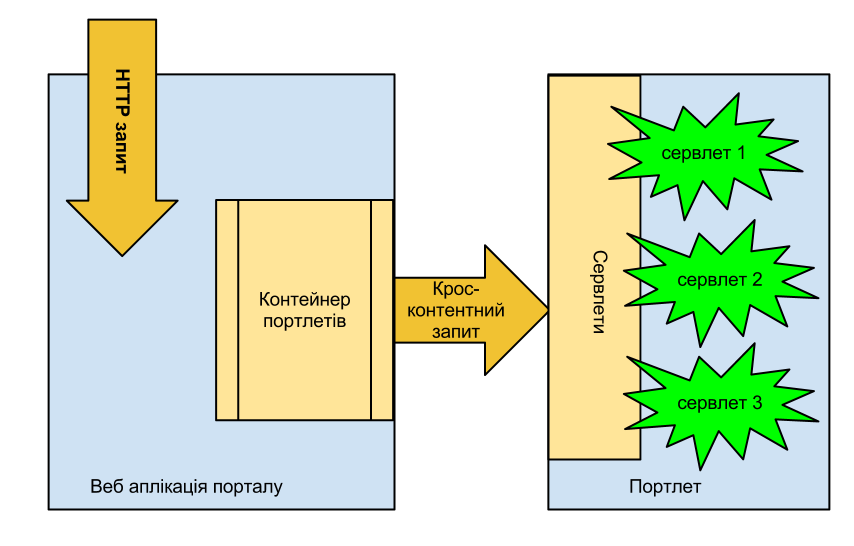
\includegraphics[width=1.00\textwidth]{pluto.png}
		\vspace{6 pt}
		\captionof{figure}{Принцип роботи Apache Pluto}\label{pic:pluto}
	\end{figure}


\par В даному випадку, Pluto вбудований безпосередньо в корпоративний портал. 
Потім через перехресний запит (через веб-додатки) відбувається відправлення запиту для відображення вмісту портлету, який як правило знаходиться в різних додатках на порталі і в контейнерах. 

\subsection{Система керування вмістом}
Система управління контентом (content management system -- CMS) дозволяє публікувати, редагувати і змінювати вміст веб-сторінок, а також обслуговувати портал з центральної сторінки. 
При цьому надається набір процедур, що використовуються для управління робочим процесом у середовищі для спільної роботи.
Вони можуть бути ручні або комп'ютеризовані (в автоматичному режимі).
\subsubsection{Головні функції CMS}
До основних функцій можна віднести наступні пункти:
\begin{itemize}
\item можливість великій кількості людей ділитися інформацією і робити свій вклад в розвиток порталу;
\item контроль доступу до даних на основі ролей користувачів (наприклад визначити роль, яка має тільки права на перегляд інформації, або ж редагування, публікацію тощо);
\item пошук і поширення інформації між користувачами;
\item зменшення дублікацій на вході;
\item спрощене керування корпоративними додатками;
\item відносно легка комунікація між користувачами.
\end{itemize}

\subsubsection{Типи даних та їх використанням}
У CMS дані можуть бути представлені як правило у будь-якій формі: документи, відео, тексти, фотографії, номери телефонів, наукові дані і тому подібне. 
CMS часто використовуються для зберігання, управління, перегляду і публікації документів. 
Також досить поширене використання в якості центрального сховища у зв'язці із централізованою системою контролю версій, що є однією із переваг CMS.
\subsubsection{Управління корпоративною інформацією}
Enterprise Content Management (ECM) -- управління інформаційними ресурсами підприємства або управління корпоративною інформацією.
В даному контексті інформація (контент) передбачається як слабо структурована одиниця -- це можуть бути файли різних форматів, електронні документи з різними наборами полів і т. п.
За визначенням ECM -- це стратегічна інфраструктура і технічна архітектура для підтримки єдиного життєвого циклу неструктурованої інформації різних типів і форматів. 
ECM-системи складаються з додатків, які можуть взаємодіяти між собою, а також використовуватися і продаватися самостійно. 
\par Всі сучасні ECM-системи визначають такі ключові компоненти:
\begin{itemize}
\item управління документами -- довгострокове архівування, автоматизація політик зберігання та відповідності нормам регулюючих органів, забезпечення відповідності законодавчим та галузевим нормам;
\item управління веб-контентом (WCM) -- автоматизація ролі веб-майстра, управління динамічним контентом і взаємодієя між користувачами;
\item  управління мультімедіаконтентом (DAM) -- управління графічними, відео та аудіофайлами, різними маркетинговими матеріалами, наприклад, флеш-банерами, рекламними роликами;
\item управління знаннями (Knowledge Management) -- підтримка систем для накопичення та доставки релевантної для бізнесу інформації;
\item документо-орієнтована взаємодія (співробітництво) -- спільне використання документів користувачами та підтримка проектних команд.
\end{itemize}

\subsection{Система управління документами}
Система управління документами (DMS -- Document management system) -- комп'ютерна система (або набір комп'ютерних програм), що використовується для відстеження та зберігання електронних документів і / або образів (зображень та інших артефактів) паперових документів.
Дане поняття тісно пов'язане з концепцією Content Management System (система керування вмістом) і зазвичай розглядається як компонента Enterprise Content Management System (CMS рівня підприємства).
У загальному випадку системи управління документами надають можливість зберігання, ведення контролю версій, позначення метаданими і безпеку по відношенню до документів, а також індексування і розвинені можливості пошуку документів.
\subsubsection{Метадані}
Метадані зазвичай зберігаються для кожного документа. 
Метадані, наприклад, можуть включати дату занесення документа в сховище і код користувача, котрий виконав зміни до файлу. 
Система управління документами також може витягувати метадані з документа автоматично або запитувати їх у користувача. 
Деякі системи надають сервіс оптичного розпізнавання тексту відсканованих документів, або можливість витягувати текст з електронних документів. 
Використовуючи опрацьований текст система дозволяє здійснювати пошук документа за ключовими словами всередині самого документа.

\subsubsection{Інтеграція }
Багато систем управління документами намагаються інтегрувати функцію управління документами безпосередньо в різні додатки, дозволяючи користувачеві отримувати документ відразу зі сховища системи управління документами, робити будь-які модифікації і зберігати його назад в сховище в якості нової версії, і все це проробляти в одному додатку, не виходячи з нього. 
Дана інтеграція в основному доступна для офісних пакетів і поштових клієнтів або для програмного забезпечення призначеного для групової або колективної роботи. 
Інтеграція зазвичай має на увазі використання таких відкритих стандартів як: ODMA, LDAP, WebDAV і SOAP.

\subsubsection{Захоплення тексту}
Під захопленням тексту мається на увазі переведення паперових документів в цифровий варіант за допомогою сканерів та багатофункціональних пристроїв.
Також часто використовується програмне забезпечення для оптичного розпізнавання тексту, щоб конвертувати цифрові зображення в текст.

\subsubsection{Індексування}
Індексування надає можливість класифікувати документи за допомогою метаданих і індексування словникового тексту, який було витягнутого з документа.
Індексація існує для підтримки розвинених можливостей пошуку документів. 
Одна з головних умов швидкого та якісного пошуку -- це створення індексу документа.

\subsubsection{Призначення сховища даних}
Основне призначення сховища даних -- це для зберігання електронних версій документів. 
Сховище документів також включає в себе і керування тими ж документами, котрі в ньому зберігаються.
Також сховище забезпечує міграцію з одного носія на інший і забезпечує цілісність даних.
Сховище документів може бути як файлове, так і сховище у вигляді СКБД (бази даних). 
У свою чергу, сховище документів в СКБД може бути як в одній базі даних, так і в окремо розподілених базах даних.
        

\subsection{Програмне забезпечення для спільної роботи}
Програмне забезпечення для спільної роботи (англ. collaborative software, groupware, workgroup support systems, group support systems) -- програмне забезпечення створене з метою підтримки взаємодії між людьми, котрі одночасно працюють над вирішенням деяких спільних завдань. 

\subsubsection{Огляд ПЗ для спільної роботи}
Програмне забезпечення для спільної роботи -- це область, яка в значній мірі перекривається з областю CSCW (англ. computer-supported cooperative work (CSCW)).
Часто вважається що ці області еквівалентні, хотя з іншого боку програмне забезпечення для спільної роботи є підчастиною CSCW.
Сюди відносяться такі системи як: електронна пошта, календарі, текстовий чат, Wiki сторінки, корпоративні закладки, блог.
Оскільки ПЗ для спільної роботи відноситься до технологічних елементів CSCW, системи спільної роботи стають корисним аналітичним інструментом у вивченні поведінкових і організаційних параметрів, пов'язаних з більш широкою сферою CSCW.

%FIXME забрати перекладений текст, хтось колись в неті перекладав
\subsubsection{Види взаємодії}
В літературі можна зустріти кілька різних визначень спільної роботи (англ. - collaboration) в застосуванні до інформаційних технологій. Деякі з них виправдані, інші ж настільки великі, що починають втрачати будь-який сенс.
Для того щоб бути впевненим що обрані технології підходять для конкретних потреб, необхідно розуміти відмінності в способах взаємодії людей один з одним.
Є три основні шляхи, по яких здійснюється взаємодія між людьми: 
\begin{itemize}
\item діалог;
\item здійснення угоди;
\item співробітництво.
\end{itemize}

\par Діалог -- це обмін інформацією між одним або кількома учасниками, основна мета якого полягає у з'ясуванні їх позицій і встановлення взаємин. 
Відбувається вільний обмін інформацією без будь-яких обмежень. 
Для підтримання діалогу цілком підходять звичайні комунікаційні технології, такі як телефон, миттєві повідомлення та електронна пошта.
\par Укладення угоди передбачає обмін деякими сутностями і ця процедура зазвичай проводиться за добре визначеними правилами і передбачає зміну відносин між учасниками. Наприклад, один з учасників угоди обмінює гроші на товари і стає покупцем. Новий статус учасників операції та обмінюваних сутностей потрібно зберегти в будь-якому надійному сховищі. Такі операції добре обслуговуються системами управління транзакціями. 
\par Співпраця полягає в тому, що його учасники обмінюються деякими загальними сутностями, на противагу угоді, коли предмет обміну належить лише одному учаснику. 
Як приклад, можна привести просування нової ідеї, створення нової конструкції, досягнення спільних цілей. 
При цьому самі сутності досить розпливчасті і невизначені. 
Таким чином, технології для забезпечення спільної роботи теж повинні бути достатньо гнучкими. 
Вони повинні включати в себе управління документами, ведення обговорень з можливістю сортування за темами, можливість відновити історію внесених змін та багато іншого.
 
\subsubsection{Рівні взаємодії}

Рівні взаємодії можна поділити на три категорії по рівню забезпечення взаємодії: засоби зв'язку, засоби для організації конференцій та засоби управління.

\par Електронні засоби зв'язку використовуються для пересилання повідомлень, файлів, даних чи документів між людьми і таким чином дають можливість для обміну інформацією:
\begin{itemize}
\item електронна пошта;
\item факс;
\item голосова пошта;
\item веб-публікації.
\end{itemize}

Електронні конференції також дають змогу для обміну інформацією, проте в інтерактивній формі це є:
\begin{itemize}
\item телефонні конференції;
\item відео і аудіо конференції;
\item Інтернет форуми;
\item чати.
\end{itemize}

Засоби управління діяльності групи:
\begin{itemize}
\item електронні календарі (створення щоденників, системи автоматичного нагадування);
\item системи управління проектами (складання розкладу робіт, відслідковування прогресу виконання);
\item управління документообігом;
\item бази знань: збір, сортування, зберігання і організація доступу до різних форм інформації.
\end{itemize}





\subsection{Інтранет}
Інтранет (англ. Intranet, також вживається термін інтрамережа) -- на відміну від мережі Інтернет, це внутрішня приватна мережа організації. 
Як правило, Інтранет -- це Інтернет в <<мініатюрі>>, який побудований на використанні протоколу IP для обміну і спільного використання деякої частини інформації всередині певної організації. 
Це можуть бути списки співробітників, списки телефонів партнерів і замовників. 
Найчастіше під цим терміном мають на увазі тільки видиму частину Інтранет -- внутрішній веб-сайт організації. 
Заснований на базових протоколах HTTP і HTTPS і організований за принципом клієнт-сервер, Інтранет-сайт доступний з будь-якого комп'ютера через браузер. 
\par Таким чином, Інтранет -- це <<приватний>> Інтернет, обмежений віртуальним простором окремо взятої організації. 
Інтранет допускає використання публічних каналів зв'язку, що входять в Інтернет, (VPN), але при цьому забезпечується захист переданих даних і присутній набір заходів щодо припинення проникнення ззовні на корпоративні вузли.
\par Програми в Інтранет засновані на застосуванні Інтернет технологій і особливо веб-технології: гіпертекст у форматі HTML, протокол передачі гіпертексту HTTP і інтерфейс серверних додатків CGI. 
Складовими частинами Інтранет є веб-сервери для статичної або динамічної публікації інформації і браузери для перегляду й інтерпретації гіпертексту.

\subsubsection{Особливості, переваги та недоліки Інтранет}
Інтранет побудований на базі тих же понять і технологій, які використовуються для Інтернету, такі як архітектура клієнт-сервер і стек протоколів Інтернету (TCP / IP). 
В Інтранеті зустрічається все з відомих Інтернет-протоколів, наприклад, протоколи HTTP (веб-служби), SMTP (електронна пошта) і FTP (передача файлів). 
Інтернет-технології часто використовуються для забезпечення сучасними інтерфейсами функцій інформаційних систем, які розміщують корпоративні дані.
\par Інтранет можна представити як приватну версію Інтернету, або як приватнe розширення Інтернету, обмеженого організацією за допомогою брандмауера. 
\par Перші Інтранет веб-сайти і домашні сторінки почали з'являтися в організаціях у 1990-1991 роках. 
Проте за неофіційними даними, термін Інтранет вперше почав використовуватися в 1992 році в таких закладах, як університети і корпорації, що працюють у технічній сфері.
\par Інтранет також протиставляють Екстранет, доступ до Інтранету надано тільки службовцям організації, в той час як до Екстранет можуть отримати доступ клієнти, постачальники, або інші затверджені керівництвом особи. 
В Екстранет-технології крім приватної мережі, користувачі мають доступ до Інтернет ресурсів, але при цьому здійснюються спеціальні заходи для безпечного доступу, авторизації, і аутентифікації.
\par Інтранет компанії не обов'язково повинен забезпечувати доступ до Інтернету. 
Коли такий доступ все ж забезпечується, зазвичай це відбувається через мережевий шлюз з брандмауером, захищаючи Інтранет від несанкціонованого зовнішнього доступу. 
Мережевий шлюз часто також здійснює аутентифікацію користувачів, шифрування даних, і часто -- можливість з'єднання по віртуальній приватній мережі (VPN) що знаходяться за межами підприємства.

Переваги використання Інтранет:
\begin{itemize}
\item висока продуктивність при спільній роботі над деякими загальними проектами;
\item легкий доступ персоналу до даних;
\item гнучкий рівень взаємодії: можна міняти бізнес-схеми взаємодії як по вертикалі, так і по горизонталі;
\item миттєва публікація даних на ресурсах Інтранет дозволяє специфічні корпоративні знання завжди підтримувати у формі і легко отримувати звідусіль в компанії, використовуючи технології мережі та гіпермедіа;
\item дозволяє проводити в життя загальну корпоративну культуру і використовувати гнучкість і універсальність сучасних інформаційних технологій для управління корпоративними роботами.
\end{itemize}


Переваги веб-сайту в Інтранет перед клієнтськими програмами архітектури клієнт-сервер:
\begin{itemize}
\item не потрібно інсталяція програми-клієнта на комп'ютерах користувачів (як неї використовується браузер);
\item відповідно, при змінах функціональності корпоративної інформаційної системи оновлення клієнтського ПЗ також не потрібно;
\item  скорочення тимчасових витрат на рутинних операціях по вводу різних даних, завдяки використанню веб-форм замість обміну даними по електронній пошті;
\item крос-платформна сумісність.% - стандартний браузер на Microsoft Windows, Mac і GNU / Linux / * NIX.
\end{itemize}


Основні недоліки Інтранет:
\begin{itemize}
\item мережа може бути зламана і використана в хакерських цілях;
\item неперевірена або неточна інформація, опублікована в Інтранет, призводить до плутанини і непорозумінь;
\item легкий доступ до корпоративних даних може спровокувати їх витік до конкурентів через несумлінного працівника;
\item працездатність і гнучкість Інтранет вимагають значних накладних витрат на розробку і адміністрування.
\end{itemize}








\subsection{Корпоративна Wiki}

Корпоративна Wiki -- це програмне забезпечення яке призначене для використання в корпоративній сфері і служить особливим чином для підвищення внутрішнього обміну знаннями, з великим акцентом на такі функції, як контроль доступу, інтеграція з іншими програмними продуктами та управління документами. 
\par В організаціях Wiki може або додати або замінити централізовану систему керування контентом. 
Її децентралізований характер дозволяє швидкому поширенню необхідної інформації в межах організації.
Вікі являється швидшим організаційним продуктом ніж централізований репозиторій знань.
Вікі може використовуватися для управління проектами, взаємодією з клієнтами, планування ресурсів підприємства а також інші види управління даними.

\par Особливості Wiki для корпорації включають в себе такі основні аспекти як:
\begin{itemize}
\item швидкий і простий доступ для створення сторінок, які містять посилання на інші корпоративні системи;
\item дозволяє розвантажити електронну пошту за рахунок зберігання всієї необхідної інформації із можливістю спільного доступу людьми які є на даному проекті;
\item гнучка організація інформації;
\item швидкий і розширений пошук.
\end{itemize}



\subsection{Онлайн офіс}
Онлайн офіс -- це набір веб-сервісів у формі програмного забезпечення яке подану кінцевому користувачеві як послуга. 
Набір наданих веб-служб зазвичай включає всі основні можливості традиційних офісних пакетів, такі як текстовий редактор, електронні таблиці, додаток для створення презентацій, органайзер справ і навіть аналоги СКБД. 
Онлайн офіс може бути доступний з будь-якого комп'ютера, у якого є доступ в Інтернет, незалежно від того, яку операційну систему користувач використовує. 
Це дозволяє людям працювати разом по всьому світу і в будь-який час, що веде до створення міжнародних віртуальних команд для спільної роботи над проектами. 


\subsection{Корпоративний блог}
Корпоративний блог -- це блог, що видається організацією і використовується як для зв'язків з громадськістю, так і для внутрішньої організації. 
Або повністю підконтрольний організації, координований і наповнюється нею контентом, але формально з нею не пов'язаний.



\subsubsection{Внутрішньокорпоративний блог}
Внутрішній корпоративний блог -- це важливий засіб комунікації, особливо у великих компаніях. 
Можна навести деякі явні переваги:
\begin{itemize}
\item блог допомагає поліпшити взаємодію співробітників, надає можливості для навчання. Він добре підходить для запуску нових проектів, для роботи в неоднорідних, великих колективах;
\item блог допомагає виявити різні погляди на будь-яке питання. Відкритість для публікації постів і коментарів -- хороша можливість висловитися всім членам колективу;
\item шляхом дискусій на задану тему блог допомагає знайти компроміс при наявності різних точок зору.
Для керівників блог -- можливість налагодити взаємодію зі співробітниками;
\item блог -- це своєрідна <<історія фірми>>, архів ідей і обговорень.
\item найчастіше кожен співробітник може залишити коментар до будь-якого посту. Коло авторів блогу визначається політикою компанії, часто написати пост може будь-який співробітник.
\end{itemize}


Блог має певні переваги перед такими внутрішньокорпоративними комунікаціями, як, наприклад, листування по електронній пошті, зокрема:

\begin{itemize}
\item коли листів стає занадто багато, це ускладнює спілкування;
\item не всі співробітники вміють правильно архівувати листи, в результаті чого вони не зможуть згодом знайти необхідну інформацію.
\end{itemize}

Внутрішній блог -- альтернатива чи доповнення до корпоративних зборів, нарад. 
Співробітники великих компаній часто не мають можливість проводити наради (наприклад, через велику відстань між філіями або зайнятості).

\subsubsection{Публічний блог}
Одна з основних цілей компаній -- це налагодження комунікацій з клієнтами.
% (як поточними, так і потенційними).
Завдяки оперативності публікації постів і можливості коментування публічний корпоративний блог дуже важливий для досягнення цієї мети.
Блоги є цінним доповненням до корпоративного сайту, так як в них може бути представлена альтернативна точка зору на те чи інше питання, ті чи інші продукти компанії можуть бути описані більш простою і доступною мовою.

\section{АЛГОРИТМІЧНЕ ЗАБЕЗПЕЧЕННЯ ПРОЦЕСУ СТВОРЕННЯ КОРПОРАТИВНОЇ СИСТЕМИ}

\subsection{Загальні вимоги до програмного продукту}
Основою будь-якої корпоративної системи є можливість можливість використання системи управління користувачами.
Тому слід розробити повний цикл взаємодії користувачів. Сюди повинні бути включені наступні такі важливі аспекти:
\begin{enumerate}
	\item можливість авторизації користувачів;
	\item ролі користувачів;
	\item зберігання даних у закодованому вигляді;
	\item чіткий розподіл прав користувачів;
	\item легка взаємодія між користувачами;
	\item можливість інтеграції із іншими сервісами системи.
\end{enumerate}

\par Тому слід розглянути кожний пункт більш детально.

\subsubsection{Авторизація користувачів}
Кожний працівник (він же користувач системи) повинний мати безперебійний доступ до свого профілю в будь-який час.  


\subsection{Проектування системи}
На початку розробки будь-якого програмного продукту слід значну увагу приділити проектування системи, адже саме від цього буде залежати легкість і правильність подальшої розробки системи, її підтримка і удосконалення.
Саме тому проектування визначає основну складову програмного забезпечення. 
Необхідні пункти для успішного запуску  продукту:
\begin{enumerate}
	\item побудова UML діаграми класів;
	\item побудова діаграми відношень між об'єктами;
	\item проектування бази даних;
	\item створення макетів майбутнього інтерфейсу;
	\item чітке розмежування модулів системи і їх взаємодія і тому подібне.
\end{enumerate}

\par Як було згадано вище, перш за все слід розробити діаграму класів, показати всі взаємовідношення між об'єктами, їх роль у системі та загальну взаємодію.
\subsubsection{Проектування UML діаграми класів}


TODO
Короче щось тут сказати про проектування, а то бошка щось не варить)))
В залежності від того, як буде спроектовано систему в цілому, буде
Додати архітектуру сайту
всякі технології опис, і буде купа сторінок:)
\subsection{Структура проекту}

\subsubsection{Проектування бази даних}
Як і кожний великий проект, даний проект повинний працювати із базою даних.

\begin{center}
		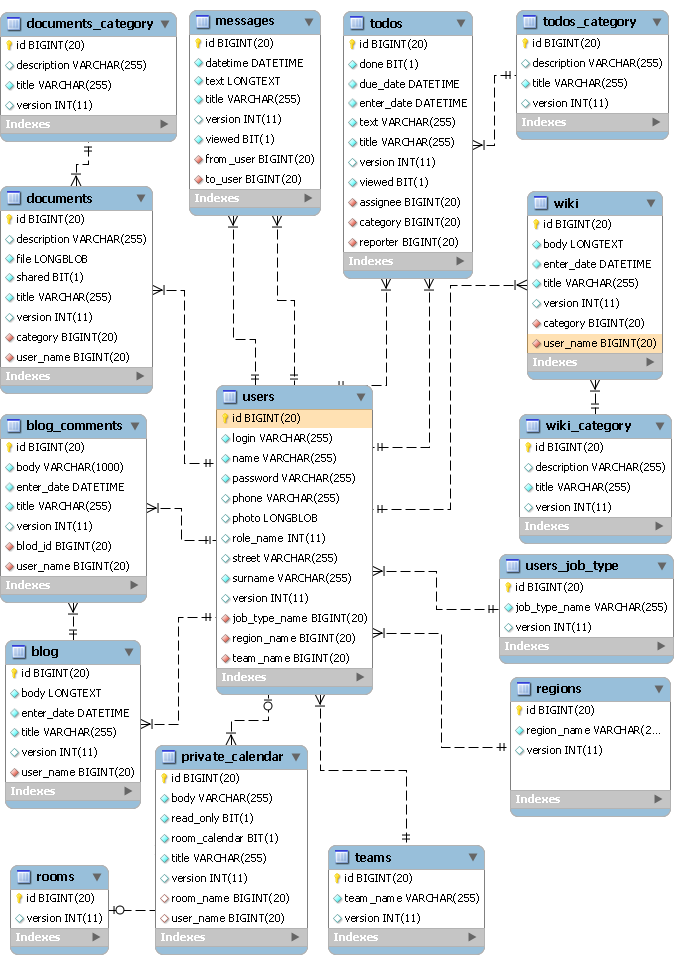
\includegraphics[width=1.00\textwidth]{db_schema.png}
		\captionof{figure}{Загальна схема структури бази даних}
\end{center}


\begin{center}
		
\includegraphics[width=1.00\textwidth]{mockup_mainpage.png}
		\captionof{figure}{Макет майбутнього сайту}
\end{center}


\begin{center}
		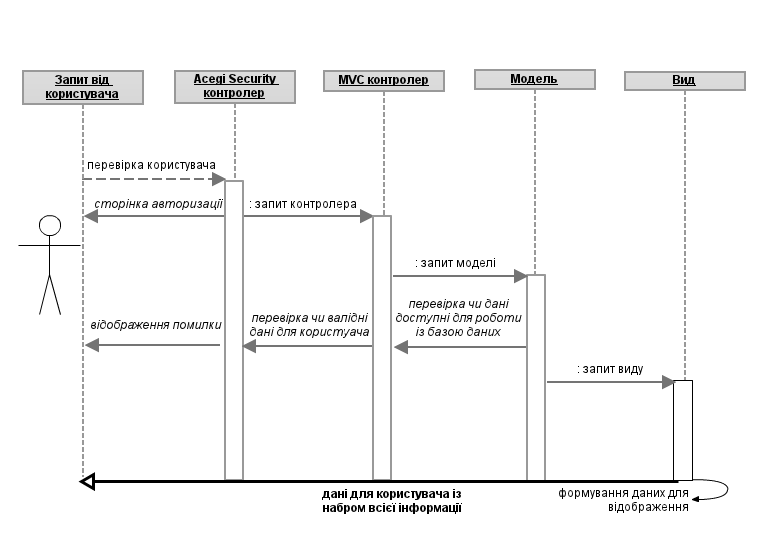
\includegraphics[width=1.00\textwidth]{sequence_diagram.png}
		\captionof{figure}{Діаграма відношення запиту користувача до роботи сервера}
\end{center}

\section{ПРОГРАМНА РЕАЛІЗАЦІЯ СИСТЕМИ ДЛЯ УПРАВЛІННЯ КОРИСТУВАЧАМИ, ДОКУМЕНТАМИ, ЗАВДАННЯМИ І МОЖЛИВОСТІ СПІЛЬНОЇ РОБОТИ}
\subsection{Реалізація роботи бази даних}
\par Загальна структура бази даних зображено на рисунку \ref{pic:db_shema}. Весь код для створення бази даних реалізовано мовою SQL, за допомогою запитів до БД.
\par Зовнішні посилання створено за допомогою команди Reference. Для прикладу код для створення таблиці користувачів (worker), котра має чотири зовнішні ключі які посилаються на таблиці команди (team), роль користувача (role\_name), тип посади (job\_type\_name) та регіон (region\_name).

\par Відповідно таким чином і реалізовано всі решта таблиць. Код для створення таблиці таблиці користувачів:
\begin{lstlisting}[language=SQL]
DROP TABLE IF EXISTS `worker`;
/*!40101 SET @saved_cs_client     = @@character_set_client */;
/*!40101 SET character_set_client = utf8 */;
CREATE TABLE `worker` (
  `id` bigint(20) NOT NULL AUTO_INCREMENT,
  `birthday` date DEFAULT NULL,
  `date_hire` date DEFAULT NULL,
  `login` varchar(255) NOT NULL,
  `name` varchar(255) NOT NULL,
  `pass` varchar(255) NOT NULL,
  `phone` varchar(255) DEFAULT NULL,
  `photo` longblob,
  `private_mail` varchar(255) DEFAULT NULL,
  `street` varchar(255) DEFAULT NULL,
  `surname` varchar(255) NOT NULL,
  `version` int(11) DEFAULT NULL,
  `job_type_name` bigint(20) NOT NULL,
  `region_name` bigint(20) NOT NULL,
  `role_name` bigint(20) DEFAULT NULL,
  `team_name` bigint(20) NOT NULL,
  `mobile` varchar(255) DEFAULT NULL,
  PRIMARY KEY (`id`),
  UNIQUE KEY `login` (`login`),
  KEY `FKD162537E30271785` (`team_name`),
  KEY `FKD162537EB0DD720C` (`job_type_name`),
  KEY `FKD162537E520C2F83` (`role_name`),
  KEY `FKD162537EBDECCB25` (`region_name`),
  CONSTRAINT `FKD162537E30271785` FOREIGN KEY (`team_name`) REFERENCES `team` (`id`),
  CONSTRAINT `FKD162537E520C2F83` FOREIGN KEY (`role_name`) REFERENCES `worker_role` (`id`),
  CONSTRAINT `FKD162537EB0DD720C` FOREIGN KEY (`job_type_name`) REFERENCES `worker_job_type` (`id`),
  CONSTRAINT `FKD162537EBDECCB25` FOREIGN KEY (`region_name`) REFERENCES `region` (`id`)
) ENGINE=InnoDB AUTO_INCREMENT=3 DEFAULT CHARSET=utf8;
/*!40101 SET character_set_client = @saved_cs_client */;	
\end{lstlisting}
\par Посилання на інші таблиці на веб інтерфейсі реалізовано за допомогою випадаючих списків -- це дає можливість забезпечити введення вірних даних і допомагає відобразити вже існуючі в базі даних записи.
Для прикладу візьмемо форму для створення нового користувача та вибору регіону, що зображено на рисунку \ref{pic:page_drop_down}.


\begin{figure}[!ht]
\centering
    
\includegraphics[width=0.5\textwidth]{page_drop_down.png}
    \captionof{figure}{Вибір регіону при створенні користувача}\label{pic:page_drop_down}
\end{figure}


\subsection{Реалізація веб інтерфейсу}
\par Веб інтерфейс користувача повинний бути зручний та інтуїтивно зрозумілий кожному користувачеві, тому його було реалізовано в легких тонах та зручно розташовано всі навігаційні елементи.

\begin{figure}[!ht]
\centering
		
\includegraphics[width=1.00\textwidth]{page_main.png}
		\captionof{figure}{Загальний інтерфейс програмного продукту}\label{pic:page_main}
\end{figure}
\par Весь інтерфейс сайту поділяється на три основні компоненти: головний блок, навігаційна панель, головне меню. Для зручності розробки цих компонентів використано Apache Tiles, що дає змогу поділяти код на логічні одиниці.
\begin{lstlisting}
<body>
 <div id="wrapper">
  <header>
   <tiles:insertAttribute name="header" ignore="true" />
  </header>
  <section>
   <div class="container_8 clearfix">
    <tiles:insertAttribute name="menu" ignore="true" />
    <tiles:insertAttribute name="body" />
   </div>
   <div id="push"><!-- --></div>
  </section>
 </div>
  <footer>
   <tiles:insertAttribute name="footer" ignore="true" />
  </footer>
 <div class="apple_overlay black" id="overlay">
  <a class="close"></a>
  <iframe class="contentWrap" style="width: 100%; height: 500px"></iframe>
 </div>
 <div style="display: none; position: absolute;" id="calroot">
  <div id="calhead">
   <a id="calprev"></a>
   <div id="caltitle"></div>
   <a id="calnext"></a>
  </div>
  <div id="calbody">
   <div id="caldays">
    <span>Sun</span><span>Mon</span><span>Tue</span><span>Wed</span><span>Thu</span><span>Fri</span><span>Sat</span>
   </div>
   <div id="calweeks">
    <!--   -->
   </div>
  </div>
 </div>
</body>
\end{lstlisting}



\subsubsection{Навігаційна панель}
\par На навігаційній панелі розташовані елементи швидкого доступу до завдань та задач.
З легкістю можна додати будь-яке завдання, при чому вибрати заголовок завдання, детальний опис та кінцевий час виконання (рисунок \ref{pic:page_navigation_new_task});
\begin{figure}[!ht]
\centering
    
\includegraphics[width=0.3\textwidth]{page_navigation_new_task.png}
    \captionof{figure}{Приклад створення завдання із навігаційної панелі}\label{pic:page_navigation_new_task}
\end{figure}
\par Для зручності навігаційна панель рухається разом із прокруткою сторінки, тобто якщо навіть користувач перейде в низ сторінки, то йому панель буде завжди доступна -- це зроблено для простоти і швидкості доступу до створення нової нотатки та завдання.
\par Справа на навігаційній панелі розташовано меню користувача. Тут знаходяться кнопки переходу на профіль робочого та кнопка виходу із сайту (рисунок \ref{pic:page_navigation_profile}). Після виходу всі дані, які збережені в сесії будуть видалені.
\begin{figure}[!ht]
\centering
    
\includegraphics[width=0.3\textwidth]{page_navigation_profile.png}
    \captionof{figure}{Панель користувача}\label{pic:page_navigation_profile}
\end{figure}


\subsubsection{Головне меню}
\par Навігація по веб ресурсу реалізована за допомогою головного меню. В головному меню відображаються всі доступні на сайті навігаційні посилання:
\begin{itemize}
  \item головна сторінка;
  \item корпоративна пошта;
  \item завдання;
  \item календар;
  \item нотатки;
  \item документи;
  \item список робочих;
  \item корпоративна вікі;
  \item блог.
\end{itemize}
\par При переході на будь-яке меню, воно зразу підсвічується -- це зроблено для зручності користувачеві, щоб було зразу видно де він знаходиться в даний момент часу. Програмно це відбувається за допомогою передачі з контролера в модель атрибута із назвою меню:
\begin{lstlisting}[language=Java]
uiModel.addAttribute("menu", "NOTE");
\end{lstlisting}
\par Потім в JSP вигляді головного меню відбувається перевірка на значення поточного меню, і якщо воно сходиться із атрибутом <<menu>> то додається css клас <<active>> (рисунок \ref{pic:page_menu}):

\begin{lstlisting}
<c:choose>
<c:when test="${menu eq 'NOTE' }"><li class="active"><a class="nav-icon icon-note" href="/ccms/notes">Notes</a></li></c:when>
<c:otherwise><li><a class="nav-icon icon-note" href="/ccms/notes">Notes</a></li></c:otherwise>
</c:choose>
\end{lstlisting}

\begin{figure}[!ht]
\centering
    
\includegraphics[width=0.30\textwidth]{page_menu.png}
    \captionof{figure}{Навігаційне меню порталу}\label{pic:page_menu}
\end{figure}
\par Відповідно до переходу на певний пункт, відбувається запит контролеру MVC, і вибірка даних із бази даних через контролер з подальшою передачею на вигляд. Для прикладу запит для запису в БД та перевірка на валідність даних:
\begin{lstlisting}
@RequestMapping(method = RequestMethod.POST, produces = "text/html")
public String create(@Valid Note note, BindingResult bindingResult, Model uiModel, HttpServletRequest httpServletRequest) {
    if (bindingResult.hasErrors()) {
        populateEditForm(uiModel, note);
        uiModel.addAttribute("menu", "NOTE");
        return "redirect:/notes";
    }
    uiModel.asMap().clear();
    note.setAuthor(Worker.getPrincipal());
    note.setDatetime(new Date());
    note.persist();
    uiModel.addAttribute("menu", "NOTE");
    return "redirect:/notes";
}
\end{lstlisting}


\subsection{Робота із даними}
\par Для маппінгу даних із форми до бази даних використовується JPA із Hibernate фреймворком поверх нього. Для кожної форми створюється певний домен (по своїй суті persistence bean), котрий за допомогою анотацій із пакету Javax дає змогу переносити об'єкти Java в базу даних (за допомогою використання мови запитів Hibernate Query Language). Для прикладу bean для запису нотаток в базу даних:
\begin{lstlisting} 
@Configurable
@Entity
public class Note {

@NotNull
private String title;

@NotNull
@Size(max = 1000000)
private String text;

@Temporal(TemporalType.TIMESTAMP)
@DateTimeFormat(style = "M-")
private Date datetime;

@ManyToOne
private Worker author;

public static TypedQuery<Note> findNotesByAuthorEquals(Worker author) {
    if (author == null)
        throw new IllegalArgumentException("The author argument is required");
    EntityManager em = Note.entityManager();
    TypedQuery<Note> q = em.createQuery("SELECT o FROM Note AS o WHERE o.author = :author ORDER by o.id DESC", Note.class);
    q.setParameter("author", author);
    return q;
}

public String getTitle() {
    return this.title;
}

public void setTitle(String title) {
    this.title = title;
}
\end{lstlisting}
\par В вище наведеному коді кожне поле має свій метод на getter та setter, що дає змогу в вибірки даних, та статичний метод <<findNotesByAuthorEquals>> для пошуку повідомлень даного автора, що дає змогу в любому місці здійснити операції щодо пошуку цих повідомлень.

\subsection{Категорії порталу}
\subsubsection{Авторизація}
\par Сторінка авторизації пропонує користувачеві ввести свій логін та пароль (рисунок \ref{pic:page_login}) та у випадку неправильних даних буде відображена помилка (рисунок \ref{pic:page_login_error})

\begin{figure}[!ht]
\centering
    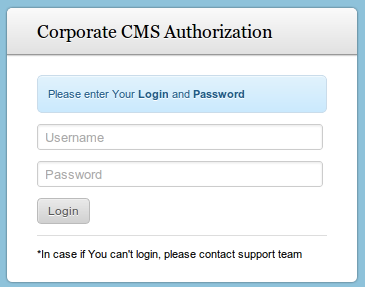
\includegraphics[width=0.50\textwidth]{page_login.png}
    \captionof{figure}{Форма авторизації користувача}\label{pic:page_login}
\end{figure}

\begin{figure}[!ht]
\centering
    
\includegraphics[width=0.50\textwidth]{page_login_error.png}
    \captionof{figure}{Помилка авторизації користувача}\label{pic:page_login_error}
\end{figure}

\par Якщо введено вірні дані, то відбувається запис нової сесії в пам'ять та перенаправлення користувача на головну сторінку, або на сторінку із якої прийшов користувач.

\subsubsection{Корпоративна пошта}
\par Всі отримані листи користувач може переглянути в пункті пошта. Напроти меню <<пошта>> відображається кількість не прочитаних повідомлень (рисунок \ref{pic:page_mail}).
  \begin{figure}[!ht]
  \centering
      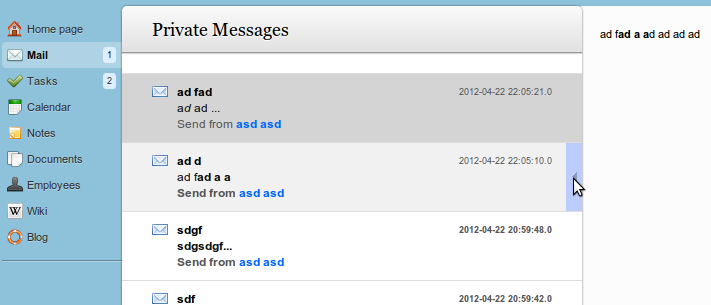
\includegraphics[width=1\textwidth]{page_mail.png}
      \captionof{figure}{Сторінка зі списком повідомлень}\label{pic:page_mail}
  \end{figure}
\par Над кожним повідомленням показано тему повідомлення. Головний текст повідомлення обрізаний, проте коли клікнути на повідомлення, збоку висунеться панель із повним описом повідомлення. Також під повідомленням показано час відправлення повідомлення та відправник повідомлення. При кліку на відправника, відбудеться перехід на його персональну сторінку. Кожне не прочитане повідомлення виділяється сирім кольором, для того щоб легше було його знайти, і при детальному перегляді його, колір забереться, і кількість повідомлень, що показуються біля меню -- буде зменшено.
\par Відправлення повідомлення можливе із персональної сторінки кожного користувача. Після переходу на персональну сторінку, слід надрукувати тему повідомлення та саме повідомлення (рисунок \ref{pic:page_send_message}).
  \begin{figure}[!ht]
  \centering
      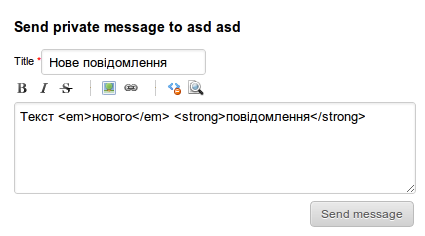
\includegraphics[width=0.8\textwidth]{page_send_message.png}
      \captionof{figure}{Форма для відправлення повідомлень}\label{pic:page_send_message}
  \end{figure}
\par Зразу також доступний wysiwyg редактор і live перегляд повідомлення яке друкується. Доставка повідомлення відбувається моментально, адже використовується локальний сервер бази даних.

\subsubsection{Календар}
Персональний календар дає змогу показати всі занесені до нього нотатки та записи. Перегляд даних можливий у трьох проміжних режимах: на місяць, на тиждень (рисунок \ref{pic:page_calendar}) та на день.
  \begin{figure}[!ht]
  \centering
      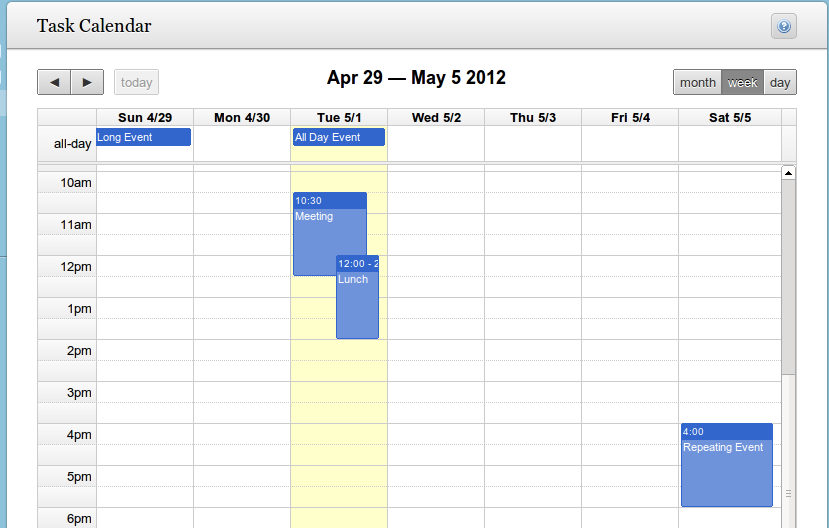
\includegraphics[width=1\textwidth]{page_calendar.png}
      \captionof{figure}{Завдання на тиждень}\label{pic:page_calendar}
  \end{figure}
\par Завдання можуть бути додані як на певний проміжний період, так і на цілий день. Для маніпуляції записів в календарі використана технологія drag \& drop від jQuery.

\subsubsection{Завдання і задачі}
\par Категорія задач створена для збереження своїх задач (\ref{pic:page_navigation_new_task}) і можливістю їх перегляду в майбутньому. Це дає змогу всі свої важливі завдання тримати в одному місці (\ref{pic:page_task}).
  \begin{figure}[!ht]
  \centering
      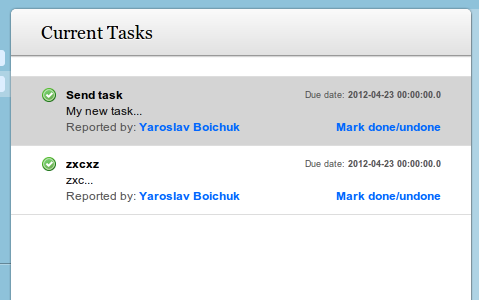
\includegraphics[width=0.7\textwidth]{page_task.png}
      \captionof{figure}{Поточні завдання}\label{pic:page_task}
  \end{figure}
\par Кожне завдання яке не виконано ще, позначається аналогічно до непрочитаного повідомлення -- сірим кольором, це дає змогу зразу побачити всі поточні завдання. Біля кожного завдання вказано хто створив дане завдання та кінцевий час його виконання. Також в головному меню навпроти пункту <<завдання>> вказується кількість невиконаних на даний момент завдань. Також кожне завдання може бути позначене як виконане або ж невиконане.

\subsubsection{Користувачі}
\par Список всіх користувачів відображається в таблиці із деяким набором полів. Для переглядаючого доступні певні маніпуляції зі списком, такі як сортування та посторінкова навігація (рисунок \ref{pic:page_workers}). А у випадку, якщо користувач наділений правами адміністратора -- то має право на створення нового користувача (рисунок \ref{pic:page_create_worker}).

  \begin{figure}[!ht]
  \centering
      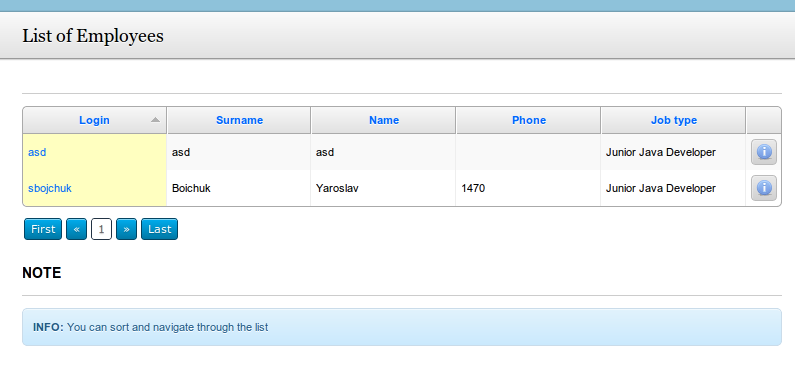
\includegraphics[width=1\textwidth]{page_workers.png}
      \captionof{figure}{Список користувачів із можливістю сортування}\label{pic:page_workers}
  \end{figure}

  \begin{figure}[!ht]
  \centering
      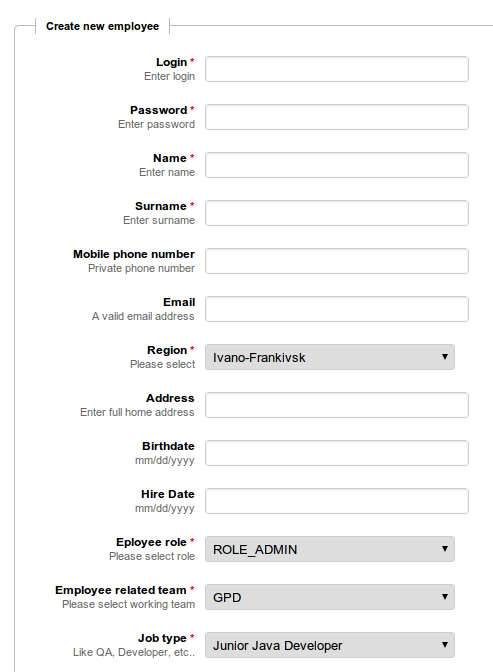
\includegraphics[width=0.7\textwidth]{page_create_worker.png}
      \captionof{figure}{Створення нового користувача}\label{pic:page_create_worker}
  \end{figure}

\par Після переходу на сторінку користувача, у його профайлі буде відображена вся детально інформація (рисунок \ref{pic:page_worker})
  \begin{figure}[!ht]
  \centering
      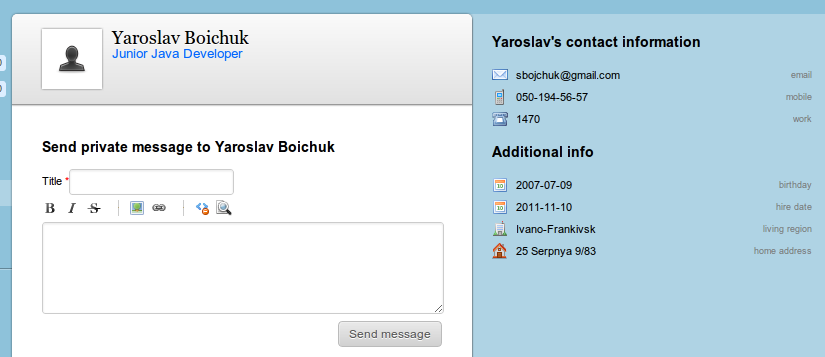
\includegraphics[width=1\textwidth]{page_worker.png}
      \captionof{figure}{Профайл користувача}\label{pic:page_worker}
  \end{figure}
\par Якщо при введенні не валідних даних, або ж залишити незаповненим обов'язкове поле -- то буде повідомлена відповідна помилка, і дані не потраплять на перевірку на сервер. Якщо ж зловмиснику вдасться все ж таки обійти перевірку форми, то сам сервер не пустить додати не валідні дані до бази даних, оскільки всі дані перевіряються другий раз за допомогою binding result об'єкта та анотації @Valid:
\begin{lstlisting}
public String update(@Valid Worker worker, BindingResult bindingResult, Model uiModel, HttpServletRequest httpServletRequest) {
if (bindingResult.hasErrors()) {
    populateEditForm(uiModel, worker);
    uiModel.addAttribute("menu", "WORKER");
    return "workers/update";
}
\end{lstlisting}
\par Якщо після проходження валідації є допущені помилка то дані назад <<повертаються>> на форму і відображається помилка. В іншому випадку, дані передадуться на модель та відбудеться запис у базу даних
\begin{lstlisting}
uiModel.asMap().clear();
worker.merge();
\end{lstlisting}


\subsubsection{Документи}
Дана категорія призначена для зберігання документів для їх спільного використання, для прикладу це можуть бути презентації, облікові документи чи просто інші нотатки. Для додавання доступні три категорії: презентації, текстові документи та таблиці. При завантаженні нового документа на портал, слід вказати категорію в котру повинен попасти документ, та вказати чи документ призначений для загально використання чи тільки для персонального.
\par Всі загальні документи доступні для завантаження та можливістю подальшого перегляду.

\subsubsection{Корпоративна wiki}
\par Корпоративна wiki в основному призначена для розповсюдження цікавої інформації між користувачами та являє собою єдине центральне сховище з можливість будь-якої маніпуляції документами. Кожна стаття має свою певну категорію -- що спрощує подальшу навігацію та пошук.

\subsubsection{Корпоративний блог}
\par Корпоративний блог має спільні риси із wiki, проте додати інформацію в нього тільки має право адміністратор та наділені такими правами групи користувачів. Основна ціль блогу -- це швидше інформування робочих про новини порталу та компанії.

\section{ЕКОНОМІЧНА ДОЦІЛЬНІСТЬ ВИКОРИСТАННЯ ПРОГРАМНОГО ЗАБЕЗПЕЧЕННЯ}

\subsection{Економічна доцільність розробки програмного забезпечення та його впровадження}

В даному проекті необхідно реалізувати корпоративну систему для спільної і одночасної роботи працівників деякої компанії. В ньому буде реалізовано систему обміну повідомленнями, управління задачами і завданнями, зручне ведення корпоративного календаря, спільна робота над документами різного типу (текстові документи, презентації тощо), система корпоративної вікі та блог. 
\par Як відомо, кожний продукт, який розробляється сьогодні з подальшим впровадженням на ринок потребує обґрунтування з економічної точки зору, а саме доцільності даного продукту. Дане обґрунтування необхідне для того, щоб вчасно припинити (при втраті актуальності або надмірних витратах) розробку або здійснити необхідні інвестування в проект для забезпечення необхідними програмними або апаратними засобами розробників з метою одержання очікуваних результатів. Економічний ефект розробленого продукту визначається на основі економічних показників, які дають можливість прогнозувати результат від впровадження даного програмного продукту.
\par Існує багато методів визначення економічних показників доцільності впровадження та використання будь-якого програмного продукту. Враховуючи інтенсивне впровадження комп’ютерної техніки в корпоративній сфері, на сьогодні такий аналіз є невід’ємною частиною попереднього аналізу аналогічних робіт, оскільки саме результат економічних показників доцільності дозволяє визначити доцільність розробки програмного продукту.
\par В даній роботі проводиться розрахунок економічних показників та аналіз всієї роботи по розробці корпоративної системи.

\subsection{Побудова мережевого графа}
Мережевий граф є основним плановим документом в системі мережевого планування і керування, що являє собою інформаційно-динамічну модель, в якій зображуються взаємозв'язки і результати всіх робіт, необхідних для досягнення кінцевої мети розробки, тобто мережевий граф -- це наочне відображення плану робіт.
\par В мережевому графі детально чи більше поверхнево показано, що, в якій послідовності, коли, за який час, для чого необхідно виконати, щоб забезпечити закінчення всіх робіт не пізніше заданого, директивного терміну.
\par Порядок побудови мережевих графів визначається прийнятою технологією і організацією робіт. Мережеві графи тільки відображають існуючу або проектовану черговість і взаємозв'язок виконання робіт.
\par По кожній роботі необхідно враховувати:
\begin{itemize}
	\item які роботи повинні бути завершені раніше, ніж почнеться дана робота;
	\item які роботи можуть початись після завершення даної роботи;
	\item які інші роботи повинні виконуватись одночасно з виконуванням даної роботи.
\end{itemize}
\par Аналізуючи мережевий граф можна виділити його головні елементи: події і роботи. Розглянемо детальніше значення термінів:
\begin{itemize}
	\item подія -- це стан, момент досягнення проміжної або кінцевої цілі розробки;
	\item робота -- це розтягнений в часі процес, необхідний для здійснення події. Кожна робота має попередню подію і закінчується визначеною подією.
\end{itemize}

\par На мережевих графах подія відображається колом, а робота -- стрілкою. До основних параметрів мережевого графа відносяться: критичний шлях, резерви часу подій. Ці параметри є вихідними для одержання ряду додаткових характеристик, а також для аналізу мережі чи для аналізу складеного плану розробки.
\par Резерв часу події -- це такий проміжок часу, на який може бути відкладене здійснення цієї події без порушення термінів завершення розробки в цілому. Резерви часу існують в мережевому графі в усіх випадках, коли існує більш ніж один шлях різної тривалості.
\par Резерв часу події $K$ визначається як різниця між пізнім $T_{p}$ і раннім $T_{r}$ термінами завершення події за формулою

\begin{equation}
	K=\frac{T_{p}}{T_{r}}
\end{equation}

\par Найбільш пізній з допустимих термінів $T_{p}$ -- це такий термін здійснення події, перевищення якого викличе аналогічну затримку завершальної події. Іншими словами, якщо подія наступила в момент $T_{p}$, вона потрапила в критичну зону і наступні за нею роботи повинні знаходитись під таким же контролем як і роботи критичного шляху.

\par Найбільш ранній з можливих термінів здійснення події $T_{p}$ -- це термін необхідний для виконання всіх робіт, що передують цій події. Цей час знаходиться шляхом вибору максимального значення із тривалості всіх шляхів, що приводять до даної події.
\par Вихідні дані мережевого графа представлені в таблицях \ref{t:eco_1} та \ref{t:eco_2}.


{\footnotesize
\begin{longtable}{|c|c|}

\captionsetup{justification=centering}
\caption{Події мережевого графа}\label{t:eco_1}\\
\hline
\multicolumn{1}{|c|}{\textbf{№ події}}&
\multicolumn{1}{c|}{\textbf{Подія}}\\\hline

\endfirsthead
\caption*{\hfill Продовження таблиці \ref{t:eco_1}}\\\hline

\multicolumn{1}{|c|}{\textbf{№ події}}&
\multicolumn{1}{c|}{\textbf{Подія}}\\\hline
\endhead

0 & Отримання завдання на дипломне проектування\\ \hline
1 & Аналіз проблеми дипломного проектування \\ \hline
2 & Ознайомлення з літературою на задану тему \\ \hline
3 & Пошук інформації в мережі INTERNET \\ \hline
4 & Підбір необхідних джерел інформації  \\ \hline
5 & Аналіз підібраного матеріалу  \\ \hline
6 & Визначення задач, які виникають при розробці  \\ \hline
7 & Розгляд існуючих способів розробки корпоративних систем \\ \hline
8 & Аналіз існуючих способів розробки  \\ \hline
9 & Пошук існуючих корпоративних систем \\ \hline
10 & Аналіз знайдених аналогів та їх функціональності \\ \hline
11 & Розробка структури алгоритму  \\ \hline
12 & Розробка алгоритму програми  \\ \hline
13 & Вибір серверної  платформи для реалізації завдання  \\ \hline
14 & Визначення основних та допоміжних програмних модулів  \\ \hline
15 & Реалізація програмних модулів в середовищі програмування  \\ \hline
16 & Попереднє налагодження програмних модулів \\ \hline
17 & Остаточне налагодження програми \\ \hline
18 & Тестування програмного продукту \\ \hline
19 & Визначення економічної доцільності використання програми \\ \hline
20 & Завершення роботи АБВГ\\ \hline

\end{longtable}
}


{\footnotesize
\begin{longtable}{|c|c|c|}
\captionsetup{justification=centering}
\caption{Роботи мережевого графа}\label{t:eco_2}\\
\hline
\multicolumn{1}{|c|}{\textbf{Номери робіт}}&
\multicolumn{1}{c|}{\textbf{Роботи}}&
\multicolumn{1}{c|}{\textbf{Тривалість, \newline дні}}\\\hline

\endfirsthead
\caption*{\hfill Продовження таблиці \ref{t:eco_2}}\\\hline

\multicolumn{1}{|c|}{\textbf{Номери робіт}}&
\multicolumn{1}{c|}{\textbf{Роботи}}&
\multicolumn{1}{c|}{\textbf{Тривалість, дні}}\\\hline
\endhead

0-1 & Аналіз завдання дипломного проекту & 2\\ \hline
1-2 & Огляд літератури & 3\\ \hline
1-3 & Огляд інформації в INTERNET & 3\\ \hline
3-4 & Робота з підібраним матеріалом з INTERNET & 4\\ \hline
2-4 & Робота з підібраним технічним матеріалом & 3\\ \hline
4-5 & Аналіз вимог до системи та її функціональності & 4\\ \hline
5-6 & Виділення та групування задач розробки & 3\\ \hline
6-7 & Пошук та розгляд існуючих методів реалізації & 7\\ \hline
7-8 & Аналіз та компонування існуючих способів розробки & 4\\ \hline
8-9 & Пошук аналогів розробленої системи & 5\\ \hline
8-10 & Аналіз аналогів розробленої системи & 4\\ \hline
9-11 & Завершення аналізу аналогів та вибір способу реалізації & 2\\ \hline
11-13 & Розробка структури алгоритму & 5\\ \hline
10-12 & Складання алгоритму програми та його аналіз & 2\\ \hline
12-13 & Розробка структури програми & 7\\ \hline
13-14 & Уточнення виду вхідних даних для програми & 5\\ \hline
14-15 & Аналіз інструментальних засобів створення програми & 2\\ \hline
15-16 & Підбір середовища програмування & 3\\ \hline
16-17 & Написання коду модулів програми & 14\\ \hline
17-18 & Налагодження всіх модулів програми & 7\\ \hline
18-19 & Завершення етапу налагодження програми & 3\\ \hline
19-20 & Тест програми та аналіз результатів тестування & 2\\ \hline
20-21 & Аналіз економічних показників & 5\\ \hline
21-22 & Завершення роботи & 14\\ \hline

\end{longtable}
}


\begin{center}
		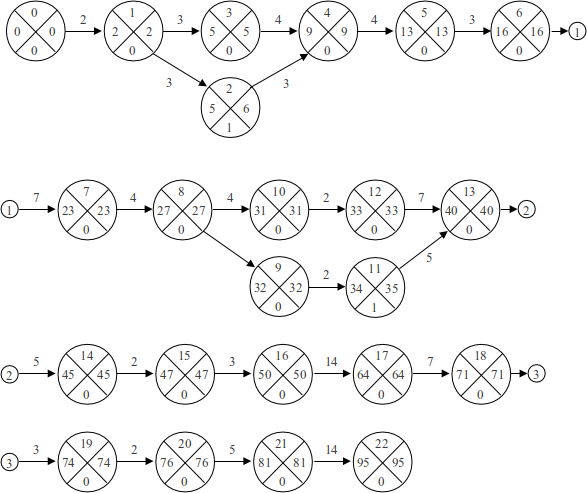
\includegraphics[width=1.00\textwidth]{ecomonic_graph.png}
		\vspace{16pt}
		\captionof{figure}{Мережевий граф виконаних робіт}\label{t:eco_graph}
\end{center}

\par На рисунку \ref{t:eco_graph} зображений мережевий граф, який отримано із вихідних даних таблиць. Знаходимо критичний шлях і розраховуємо ранній, пізній час і резерв часу.
\par Критичний шлях --- це найбільш тривала по часу послідовність робіт, які ведуть від вихідної до завершальної події. Величина критичного шляху визначає термін виконання всього комплексу по плануванню робіт.
\par Зміна тривалості будь-якої роботи, що лежить на критичному шляху, відповідним чином змінює термін настання завершальної події, тобто дату досягнення кінцевої мети, яка ставиться при плануванні розробки.
\par При плануванні комплексу операцій критичний шлях дозволяє знайти термін настання завершальної події. В процесі керування ходом розробки увага керівництва зосереджується на роботах критичного шляху. Це дозволяє найбільш  доцільно   і   оперативно  контролювати   обмежене  число  робіт, що впливають на термін розробки, а також краще використати існуючі ресурси.
\par Оскільки в даному випадку мережевий граф досить простий, очевидно що критичний шлях рівний 95.
\par Дані розрахунків часу подій приведені в таблиці \ref{t:eco_3}.


{\footnotesize
\begin{longtable}{|c|c|c|c|}

\captionsetup{justification=centering}
\caption{Параметри подій мережевого графіка}\label{t:eco_3}\\
\hline
\multicolumn{1}{|c|}{\textbf{№ події}}&
\multicolumn{1}{c|}{\textbf{Ранній час}}&
\multicolumn{1}{c|}{\textbf{Пізній час}}&
\multicolumn{1}{c|}{\textbf{Резерв часу}}\\\hline

\endfirsthead
\caption*{\hfill Продовження таблиці \ref{t:eco_3}}\\\hline

\multicolumn{1}{|c|}{\textbf{№ події}}&
\multicolumn{1}{c|}{\textbf{Ранній час}}&
\multicolumn{1}{c|}{\textbf{Пізній час}}&
\multicolumn{1}{c|}{\textbf{Резерв часу}}\\\hline
\endhead

0 & 0 & 0 & 0\\ \hline
1 & 2 & 2 & 0\\ \hline
2 & 5 & 6 & 1\\ \hline
3 & 5 & 5 & 0\\ \hline
4 & 9 & 9 & 0\\ \hline
5 & 13 & 13 & 0\\ \hline
6 & 16 & 16 & 0\\ \hline
7 & 23 & 23 & 0\\ \hline
8 & 27 & 27 & 0\\ \hline
9 & 32 & 32 & 0\\ \hline
10 & 31 & 31 & 0\\ \hline
11 & 34 & 35 & 1\\ \hline
12 & 33 & 33 & 0\\ \hline
13 & 40 & 40 & 0\\ \hline
14 & 45 & 45 & 0\\ \hline
15 & 47 & 47 & 0\\ \hline
16 & 50 & 50 & 0\\ \hline
17 & 64 & 64 & 0\\ \hline
18 & 71 & 71 & 0\\ \hline
19 & 74 & 74 & 0\\ \hline
20 & 76 & 76 & 0\\ \hline
21 & 81 & 81 & 0\\ \hline
22 & 95 & 95 & 0\\ \hline

\end{longtable}}

\subsection{Економічне обґрунтування розробки та впровадження програми}
Економічне обґрунтування розробки та впровадження програми будемо здійснювати на аналізі таких економічних показників:
\par $S_{po}$ -- сумарні витрати на розробку програмного забезпечення;
\par $\Delta{E_{e2/1}}$ -- експлуатаційні витрати.
\par Розрахунок відповідних коефіцієнтів проводиться з врахуванням того, що варіаційні задачі діагностування раніше виконувались вручну.

\subsubsection{Розрахунок витрат на розробку програмного забезпечення}
Сумарні витрати на розробку програмного забезпечення $S_{po}$ визначаються за формулою:
\begin{equation}
	S_{po} = \sum_{i}t_{po_{i}}\cdot{B_{po_{i}}}\cdot{[(1+\omega_{d})\cdot{(1+\omega_{c})}+\omega_{n}]}+t_{mo}\cdot{e_{g}},
\end{equation}
\par де $t_{po_{i}}$ -- час, що витрачається на розробку даної програми працівником $i-$ої кваліфікації, люд.-міс;
\par $B_{po_{i}}$ -- основна заробітна плата розробника $i-$-ої кваліфікації, грн/міс;
\par $\omega_{d}$ -- коефіцієнт, що враховує додаткову заробітну плату розробникам програми, у відсотках від основної заробітної плати;
\par $\omega_{c}$ -- коефіцієнт, що враховує нарахування органам соціального захисту на заробітну плату, у відсотках від основної та додаткової заробітної плати;
\par $\omega_{n}$ -- коефіцієнт, що враховує накладні витрати установи, в якій розробляється ця програма, у відсотках до основної заробітної плати розробника;
\par $t_{mo}$ -- машинний час ЕОМ, необхідний для налагоджування даної програми, машино-год;
\par $e_{g}$ -- експлуатаційні витрати, що припадають на 1 год машинного часу.

\par Значення коефіцієнтів $\omega_{d}=0$; $\omega_{c}=0.375$; $\omega_{n}=0.42$. Нехай $t_{mo}$ = 1 люд.-міс, а $B_{po_{i}}$ = 3000 грн. Експлуатаційні витрати, що припадають на 1 год машинного часу, можуть бути визначені за витратою електроенергії:

\begin{equation}\label{eq:eco_eq_3}
	S_{g} = P_{cp}\cdot{C_{bod}},
\end{equation}
\par де $P_{cp}$ = 90 Вт -- споживана потужність ЕОМ (ноутбук);
\par $C_{bod}$ = 0.8762 -- вартість 1 кВт/год електроенергії для підприємств.

\par Отже, за \eqref{eq:eco_eq_3}:
\begin{center}
	\center{$e_{g} = 0.09\cdot{0.8762}=0,079$ грн/год.}
\end{center}

\par Необхідний час налагодження програми становить 24 машино-год.
\par Сумарні витрати на розробку програмного забезпечення складуть:
	\par
\begin{center}
	$S_{po} = 1\cdot3000\cdot((1+0)\cdot(1+0.375)+0.42)+24\cdot0.079=5386.90$ грн.
\end{center}
\par Використання запропонованої програми не потребує додаткових капітальних вкладень у користувача.


\subsubsection{Розрахунок можливого прибутку}
\par Даний продукт буде розповсюджуватися за ліцензією GNU General Public License, що означає безкоштовне його розповсюдження. Тому для того щоб повернути витрачені кошти на його розробку і підтримку, варто використовувати загальні методи поширення open source програм, це заробіток на підтримці користувачів продукту (супорт). 
\par Буде введено два тарифи: річна підписка (2000 грн.), та помісячна (200 грн.).
\par Прогнози, зроблені на основі дослідження ринку, дозволяють нам очікувати наступний прибуток за 1 рік підтримки користувачів продукту на ринку. Середня кількість компаній за рік буде становити порядку 10-ти. В середньому на ринку, кожна друга компанія буде користуватися послугою супорту і налаштування продукту. Решта половина буде тільки використовувати разову місячну передплату. Отже очікуваний прибуток за 1 рік на ринку буде становити:
\par 5 місячний передплат -- $5\cdot200 = 1000$ грн.
\par 5 річних передплат -- $5\cdot2000 = 10000$ грн.
\par Очікуваний прибуток за рік становитиме: 
\par $P = (10000+1000)-5386.90 = 5613.1$ грн.
\par Чистий прибуток: $P_{ch.} = (1-0.21)\cdot5613.1=4434.35$ грн.
\par Чистий місячний прибуток буде становити: $P_{m.ch.}=369.53$ грн.


\subsubsection{Розрахунок зведених економічних показників}
\par Термін   окупності   додаткових   капітальних   вкладень   визначається   за формулою:
\begin{equation}\label{eq:eco_eq_4}
	T_{OK} = \frac{S_{po}}{P_{ch.}}
\end{equation}
\par Отже, за \eqref{eq:eco_eq_4}
\begin{center}
	$T_{OK}=5386.90/369.53=14.5$ місяця.
\end{center}

\par Ефект, який отримує корпорація при користуванні даним продуктом полягає у легкості і гнучкості взаємодії між користувачами, спільною роботу над документами і завданнями.
\par В таблиці \ref{t:eco_4} наведені зведені економічні показники системи. З вище наведених розрахунків видно, що розробка та впровадження даної програми є економічно доцільною. 


{\footnotesize
\begin{longtable}{|c|c|c|c|}

\captionsetup{justification=centering}
\caption{Зведені економічні показники розробки системи}\label{t:eco_4}\\
\hline
\multicolumn{1}{|c|}{\textbf{Показник}}&
\multicolumn{1}{c|}{\textbf{Розмірність}}&
\multicolumn{1}{c|}{\textbf{Значення}}\\\hline

\endfirsthead
\caption*{\hfill Продовження таблиці \ref{t:eco_4}}\\\hline

\multicolumn{1}{|c|}{\textbf{Показник}}&
\multicolumn{1}{c|}{\textbf{Розмірність}}&
\multicolumn{1}{c|}{\textbf{Значення}}\\\hline
\endhead

Витрати на розробку програмного забезпечення & грн & 5386.90 \\ \hline
Очікуваний економічний ефект (за рік) & грн & 4434.35 \\ \hline
Термін окупності розробки корпоративного порталу & місяць & 14.5 \\ \hline

\end{longtable}
}

\par Таким чином, з цих економічних розрахунків випливає, що розробка корпоративної системи, розповсюдження якої базується на ліцензії GNU є економічно доцільним і дозволяє отримувати прибутки від підтримки користувачів і налаштування ПЗ.
\section{ОХОРОНА ПРАЦІ}
\subsection{Значення охорони праці для забезпечення безпечних і здорових умов праці}
\par Значення охорони праці в будь-якій галузі України є дуже вагоме, адже саме охорона праці напряму пов'язана з вивченням та вирішенням питань безпеки праці на виробництві, попередженні виробничого травматизму і професійних захворювань, пожеж та вибухів, а також охорони навколишнього середовища.
\par При проведенні робіт нерідко порушуються діючі правила й інструкції з техніки безпеки. Це відбувається по причині незадовільного інструктажу й навчання робітників,  внаслідок неправильної організації робіт, недостатнього технічного нагляду зі сторони інженерно-технічних працівників.
\par Охорона праці та навколишнього середовища здійснюється на основі правових норм України і розглядає основи наукової організації праці робітників системи буріння нафтових і газових свердловин, питання виробничої санітарії, основи електробезпеки і техніки безпеки при монтажі і експлуатації бурового обладнання, моніторингу за роботою електороустановок на бурових, збором інформації з вимірювальних приладів бурових, що є важливим. 
\par Для того щоб максимально знизити травматизм, необхідна висока кваліфікація робітників, знання технологічних особливостей процесу буріння свердловин, призначення, конструкції та правила експлуатації устаткування й механізмів, правильних й безпечних прийомів виконання робіт, а також високий рівень технічного нагляду зі сторони керівників робіт.
\par Покращення організації праці, механізації тяжких й трудомістких робіт, раціоналізація технологічних процесів, впровадження нових, більш сучасних видів устаткування, механізмів та інструменту — основний напрям  підвищення продуктивності праці й створення здорової і безпечної виробничої обстановки на бурових підприємствах.

\subsection{Аналіз потенційних небезпек та шкідливих факторів виробничого середовища}

\par Важливою умовою функціонування будь-якого сучасного підриємства є робота із ЕОМ(електронно-обчислювальними машинами). Проте ця робота супроводжується впливом багатьох чиннів на організм оператора по роботі з ЕОМ. Було проведено аналіз і зроблено характеристику несприятливих виробничих факторів, які здатні впливати на здоров'я та самопочуття працівника. Всі дані наведено в таблиці \ref{t:safety1}.

{\footnotesize
\begin{longtable}{|p{4cm}|p{12cm}|}
\captionsetup{justification=centering}
\caption{Аналіз потенційних небезпек виробничих факторів при роботі з ЕОМ}\label{t:safety1}\\
\hline
\multicolumn{1}{|c|}{\textbf{Джерело небезпек}}&
\multicolumn{1}{p{12cm}|}{\textbf{Характеристика потенційно-небезпечних виробничих факторів та їх допустимі значення}}\\\hline

\endfirsthead
\caption*{\hfill Продовження таблиці \ref{t:safety1}}\\\hline

\multicolumn{1}{|c|}{\textbf{Джерело небезпек}}&
\multicolumn{1}{p{12cm}|}{\textbf{Характеристика потенційно-небезпечних виробничих факторів та їх допустимі значення}}\\\hline
\endhead

ренгенівське випромінювання	& Фактичні (середні) дані вимірів 9-12мкР/год (в діапазоні 1.2КеВ). Гранично допустима експозиційна доза: 100мкР/год.  	\\ \hline


ультрафіолетове випромінювання & Фактичні дані вимірів: 0.001 Вт/м$^2$ в діапазоні 280-315 нм - УФ-Ф). Допустима інтенсивність: 0.01 Вт$^2$ -- УФ-В\\ \hline


ІЧ-випромінювання 	& 	Фактичні дані вимірів інтенсивності теплового випромінювання 0,05-4 Вт/м$^2$ (в діапазоні 700 нм-1мм). Допустима інтенсивність:  35-70 Вт/м$^2$.	\\ \hline

видимий діапазон  	& 	Фактичні дані: 0,1-2 Вт/м$^2$ (в діапазоні 320-400 нм) і 2,5-4 Вт/м$^2$ (в діапазоні 400-700 нм). Допустима інтенсивність потоку енергії:  10 Вт/м$^2$.	\\ \hline


яскравість 	& 	Фактичні дані: 306 кд/м$^2$. Допустиме значення: 35 кд/м$^2$.	\\ \hline

електростатичне поле & Фактичні дані: 15 кВ/м (0 Гц) Допустима напруженість поля  20-60 кВ/м.\\ \hline

шум 	& 	Діюче значення звукового тиску: 28.6-44 дБА. Допустиме значення: 55дБА
	\\ \hline

\end{longtable}
}

\par Робота оператора з ЕОМ вимагає максимальної концентрації протягом цілого робочого дня, що в свою чергу призводить до значних навантажень на організм. Також через постійне розумове навантаження зростає ризик перевантаження аналізаторів та ймовірність психічного розладу.



\subsection{Забезпечення нормальних умов праці при роботі з ЕОМ}
\par Для забезпечення нормальних умов праці оператора з ЕОМ потрібно створити максимально комфортні умови праці. Для цього було обрано робочий кабінет, який відповідає всім вимогам та стандартам праці.
\par В робочому кабінеті будуть знаходитися 11 робочих місць (рисунок \ref{pic:safety_room}). На кожного працівника розраховано одна одиниця техніки (сюди входить монітор, системний блок, клавіатура, мишка). Проте деякі працівники, у зв'язку зі специфічним видом роботи, потребуються два монітори, які розташовані поряд один з один. Кожний працівник відгороджений від інших дерев'яною перегородкою. Кожний працівник забезпечений робочим місцем загальною площею 8м$^2$. 

\begin{figure}[!ht]
\centering
		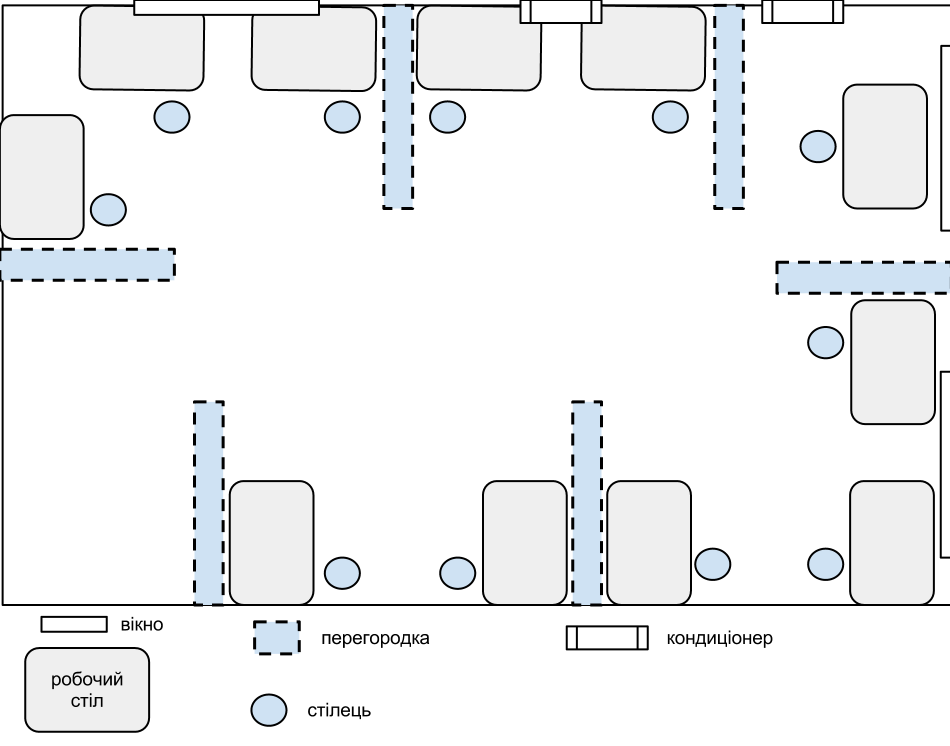
\includegraphics[width=1\textwidth]{safety_room.png}
		\vspace{18pt}
		\captionof{figure}{Схема робочої кімнати - офісу}\label{pic:safety_room}
\end{figure}

\par Також для кожного працівника, для того щоб забезпечити комфортні умови праці розраховано три висувні ящики та тумбочку для власних речей, та шафки зверху робочого місця, для швидкого доступу до документації та канцелярських речей, що в свою чергу становить загальний об'ємом 22м$^3$. Кожний працівник забезпечується зручним та комфортним кріслом, яке регулюється згідно вимог. Все це зроблено із урахуванням ГОСТ 12.2.032-78\cite{safety_g_1}, ДНАОП 0.00-1.31-99\cite{safety_g_2} та ДСан ПіН 3.3.2.007-98\cite{safety_g_3}.

\par На кожному вікні є жалюзі, що дає змогу зменшити вплив сонячних променів на працюючого (засліплення монітору для прикладу).
\par Комп'ютерна-та електромережа прокладена із врахуванням всіх вимог техніки безпеки.
\par Крім обчислювальних одиниць, більше технічних засобів в кімнаті не передбачається, адже всі переферійні пристрої розташовані на коридорі.

\par Для забезпечення мікрокліматичних умов праці передбачено два кондиціонери, які можуть працювати в автоматичному режимі і підтримувати сталу температуру приміщення. Також налагоджено роботу постійної вентиляція , яка працює за наступним принципом: вентиляційні витяжки розміщені в 4 місцях (по кутах) кімнати. Дві із них працюють як витяжки, тобто втягують повітря, інші дві забезпечують свіжим повітрям кімнату -- в кінцевому результаті постійна циркуляція повітря. Вентиляційні труби виведені на вулицю. В таблиці \ref{t:safety_microclimate} наведено оптимальні значення метеорологічних умов згідно ГОСТ 12.1.005-88 \cite{safety_gost_air} в робочому кабінеті.


{\footnotesize
\begin{longtable}{|c|c|c|c|c|}
\captionsetup{justification=centering}
\caption{Оптимальні значення метеорологічних умов в робочому кабінеті для легкої категорії робіт в офісному приміщенні}\label{t:safety_microclimate}\\
\hline
\multicolumn{1}{|c|}{\textbf{Категорія робіт}}&
\multicolumn{1}{c|}{\textbf{Період року}}&
\multicolumn{1}{c|}{\textbf{Температура, $^{\circ}$C}}&
\multicolumn{1}{c|}{\textbf{Відносна вологість, \%}}&
\multicolumn{1}{p{2.5cm}|}{\textbf{Швидкість руху повітря, м/с}}\\ \hline

\endfirsthead
\caption*{\hfill Продовження таблиці \ref{t:safety_microclimate}}\\ \hline

\multicolumn{1}{|c|}{\textbf{Категорія робіт}}&
\multicolumn{1}{c|}{\textbf{Період року}}&
\multicolumn{1}{c|}{\textbf{Температура, $^{\circ}$C}}&
\multicolumn{1}{c|}{\textbf{Відносна вологість, \%}}&
\multicolumn{1}{p{2.5cm}|}{\textbf{Швидкість руху повітря, м/с}}\\ \hline
\endhead
Легка Іа & Холодний & 22-24 & 40-60 & 0,1  \\ \hline
Легка Іа & Теплий & 23-25 & 40-60 & 0,1  \\ \hline
\end{longtable}
}

\par Як згадувалося вище про вентиляцію -- саме вентиляція є основою забезпечення комфортних умов праці, тобто регуляцію мікроклімату. Характеристику штучної вентиляції наведено в таблиці \ref{t:safety_ventil}

{\footnotesize
\begin{longtable}{|c|c|c|c|}
\captionsetup{justification=centering}
\caption{{Характеристика штучної вентиляції}}\label{t:safety_ventil}\\
\hline
\multicolumn{1}{|c|}{\textbf{Приміщення}}&
\multicolumn{1}{c|}{\textbf{Тип вентиляції}}&
\multicolumn{1}{c|}{\textbf{Вентиляційне обладнання}}&
\multicolumn{1}{p{3cm}|}{\textbf{Кратність повітряного обміну, 1/год }}\\ \hline

\endfirsthead
\caption*{\hfill Продовження таблиці \ref{t:safety_ventil}}\\ \hline

\multicolumn{1}{|c|}{\textbf{Приміщення}}&
\multicolumn{1}{c|}{\textbf{Тип вентиляції}}&
\multicolumn{1}{c|}{\textbf{Вентиляційне обладнання}}&
\multicolumn{1}{p{3cm}|}{\textbf{Кратність повітробміну, 1/год }}\\ \hline
\endhead
Офіс & Механічна & Кондиціонер (700-1000 м$^3$/год, 4 кВт), 2шт & 4.4 \\ \hline
\end{longtable}
}

\par Так як робота людини з ЕОМ більше як на 90\% складається із зорової роботи -- тому правильне і раціональне освітлення становить основу для створення сприятливих умов праці та унеможливлення розвитку професійних захворювань. Освітлення повинне забезпечувати комфортну роботу працівника в будь-яку пору дня, чи то ранок, чи обід чи вечір. Характеристика штучної освітленості робочих місць
наводиться у таблиці \ref{t:safety_shtychno} згідно ДБН В.2.5-28-2006 \cite{safety_light}.

{\footnotesize
\begin{longtable}{|c|c|c|c|c|c|}
\captionsetup{justification=centering}
\caption{Оптимальні значення метеорологічних умов в робочому кабінеті для легкої категорії робіт}\label{t:safety_shtychno}\\
\hline
\multicolumn{1}{|c|}{\textbf{Приміщення}}&
\multicolumn{1}{p{2cm}|}{\textbf{Розряд зорової роботи}}&
\multicolumn{1}{p{2cm}|}{\textbf{Загальне освітлення, лК}}&
\multicolumn{1}{p{2.5cm}|}{\textbf{Комбіноване освітлення, лК}}&
\multicolumn{1}{p{2.5cm}|}{\textbf{Аварійне освітлення для евакуації, лК}}\\ \hline

\endfirsthead
\caption*{\hfill Продовження таблиці \ref{t:safety_shtychno}}\\ \hline

\multicolumn{1}{|c|}{\textbf{Приміщення}}&
\multicolumn{1}{p{2cm}|}{\textbf{Розряд зорової роботи}}&
\multicolumn{1}{p{2cm}|}{\textbf{Загальне освітлення, лК}}&
\multicolumn{1}{p{2.5cm}|}{\textbf{Комбіноване освітлення, лК}}&
\multicolumn{1}{p{2.5cm}|}{\textbf{Аварійне освітлення для евакуації, лК}}\\ \hline
\endhead
Офіс & IVв & 200 & 400 & 0.5\\ \hline
\end{longtable}
}

\par Засоби індивідуального захисту не передбачаються, так як монітори побудовані на основі рідких кристалів, тому тут немає регенерації картинки, потім завжди сталий.



\subsection{Забезпечення безпеки монтажу, пусконалагоджувальних, ремонтних робіт та експлуатації ЕОМ і комп’ютерних мереж}

\par Так як ЕОМ завжди підключені до мережі і створюють значне навантаження неї, правильне проектування мережі визначає безпеку роботи як працівників так і самого підприємства.
\par Для забезпечення захисту людей від ураження електричним струмом використовуються окремо або в поєднанні один з одним такі технічні способи та засоби як: захисне заземлення, занулення, вирівнювання потенціалів, мала напруга, захисне відімкнення, ізоляція провідників із струмом, огороджувальні пристрої, попереджувальна сигналізація, блокування, знаки безпеки, засоби захисту та запобіжні пристрої.
\par Для захисту від дотику до частин, що знаходяться під напругою, використовується ізоляція Для захисту від дотику до частин, що знаходяться під напругою, використовується також подвійна ізоляція - електрична ізоляція, що складається з робочої та додаткової ізоляції.
\par Також передбачене використання звукової та світлової сигналізації, надписів, плакатів та інших засобів інформації, що попереджують про небезпеку.

\par Вимоги електричної і механічної безпеки для ЕОМ і систем обробки даних встановлені ГОСТ 25861 - 83 \cite{safety_gost_25861}. Додаткові або особливі заходи безпеки, яких необхідно дотримуватися при експлуатації і технічному обслуговуванні ЕОМ і їх пристроїв, вказані в ЕД (експлуатаційна документація).
\par Особи, що допускаються до експлуатації і технічного обслуговування ЕОМ, проходять цільове навчання по вивченню правил роботи і вимог безпеки при роботі з ЕОМ, а також експлуатаційну документацію на конкретні види ЕОМ, до роботи з якими вони одержують допуск. До експлуатації ЕОМ допускаються особи, що мають групу по електробезпеці не нижче II, до технічного обслуговування -- групу ІІІ.
\par Для безпечної експлуатації ЕОМ в приміщенні, де вона встановлена, забезпечуються кліматичні умови, встановлені експлуатаційною документацією.
\par Всі пристрої ЕОМ підлягають захисному заземленню, за винятком пересувних і переносних, в конструкціях яких заземлення не передбачено.

\subsection{Пожежна безпека та безпека в надзвичайних ситуаціях}
\par Згідно з ПУЕ приміщення, де експлуатуються ЕОМ і ПЕОМ, належать до приміщень без підвищеної небезпеки ураження людини електричним струмом.
\par Вимоги електробезпеки і пожежної безпеки у приміщеннях, де встановлені ЕОМ і ПЕОМ, подані у НПАОП 0.00-1.28-10 \cite{safety_gost_npaop}: ЕОМ і все устаткування для обслуговування, ремонту та налагодження їх роботи, електропроводи і кабелі мають відповідати вимогам електробезпеки зони за ПВЕ та мати апаратуру захисту від струму короткого замикання.

\par Забезпечено неможливість виникнення джерела загорання внаслідок короткого замикання та перевантаження проводів використанням негорючої ізоляції.

\par Всі приміщення обладнані системою автоматичної пожежної сигналізації з димовими пожежними сповіщувачами та двома переносними вуглекислотними вогнегасниками з зарядом вогнегасної речовини 5л. \cite{safety_vogon_nakaz} (таблиця \ref{t:safety_vogon}).

\par Всюди, включаючи коридори, передбачені засоби пожежної сигналізації на випадок НС.

\par Дані про первинні засоби пожежогасіння в офісі приводяться в таблиці \ref{t:safety_vogon}

{\footnotesize
\begin{longtable}{|c|c|c|c|c|c|}
\captionsetup{justification=centering}
\caption{первинні засоби пожежогасіння}\label{t:safety_vogon}\\
\hline
\multicolumn{1}{|c|}{\textbf{Категорія}}&
\multicolumn{1}{p{2cm}|}{\textbf{Захищена площа, м$^2$}}&
\multicolumn{1}{p{3cm}|}{\textbf{Вуглекислотний вогнегасник}}&
\multicolumn{1}{p{2cm}|}{\textbf{Хімічно-пінний вогнегасник}}&
\multicolumn{1}{p{3cm}|}{\textbf{Порошковий вогнегасник}}\\ \hline

\endfirsthead
\caption*{\hfill Продовження таблиці \ref{t:safety_vogon}}\\ \hline

\multicolumn{1}{|c|}{\textbf{Категорія}}&
\multicolumn{1}{p{2cm}|}{\textbf{Захищена площа, м$^2$}}&
\multicolumn{1}{p{3cm}|}{\textbf{Вуглекислотний вогнегасник}}&
\multicolumn{1}{p{2cm}|}{\textbf{Хімічно-пінний вогнегасник}}&
\multicolumn{1}{p{3cm}|}{\textbf{Порошковий вогнегасник}}\\ \hline
\endhead

Д & 90 & 2 & - & -  \\ \hline
\end{longtable}
}

\par З таблиці \ref{t:safety_vogon} категорія <<Д>> визначається як: <<Негорючі речовини та матеріали в холодному стані>>.

\par Для запобігання впливу на людей небезпечних чинників пожежі повинна бути передбачена можливість швидкої евакуації людей з будівлі.
\par Необхідний час для евакуації для приміщень категорії <<Д>> не обмежується.
\par Розрахунковий час евакуації визначається по розрахунку часу руху одного або декількох людських потоків через евакуаційні виходи з найбільш віддалених місць розміщення людей.

\begin{figure}[!ht]
\centering
		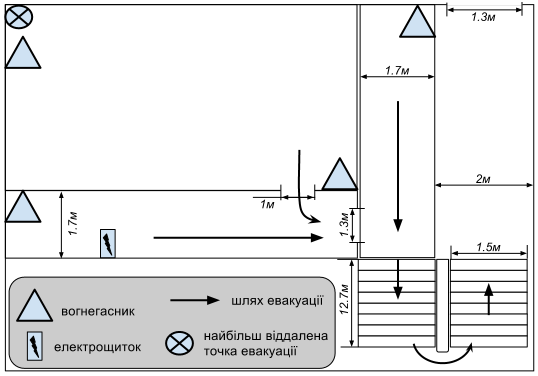
\includegraphics[width=1\textwidth]{safety_evacuation.png}
		\vspace{18pt}
		\captionof{figure}{Схема евакуації з офісу при пожежі}\label{pic:safety_evacuation}
\end{figure}

\par При розрахунку весь шлях руху людського потоку поділяється на дільниці.
\par Розрахунковий час евакуації людей потрібно визначити як суму часу руху людського потоку по окремих дільницях шляху:
	\begin{equation}
		T_{p}=T_{1}+T_{2}+ ... + T_{i},
	\end{equation}
\par де $T_{1}$ -- час руху людського потоку на першій дільниці;
\par $T_{1}, T_{1}, ..., T_{i}$ -- час руху людського потоку на кожному з наступних дільниць шляху.

\par Швидкість руху людського потоку на дільницях шляху визначається в залежності від щільності людського потоку Dn:
	\begin{equation}
		D_{n}=\frac{N_{n}\cdot f}{L_{n}\cdot S_{n}},
	\end{equation}
\par де $N_{n}$ -- число людей в відділі;
\par $f$ -- середня площа горизонтальної проекції людини, м$^2$ (в зимовий час $f = 0.125$ м$^2$, в літній час $f = 0.1$ м$^2$), приймаємо $f = 0.125$ м$^2$;
\par $L_{n}$ -- довжина дільниці шляху, м;
\par $S$ -- ширина дільниці шляху, м.

\par Далі підраховуємо час руху людського потоку на дільниці шляху:
	\begin{equation}
		T_{n}=\frac{L_{n}}{V_{n}}.
	\end{equation}

\par Інтенсивність руху людського потоку по кожному з дільниць визначаються по формулі:
	\begin{equation}
		q_{i}=\frac{q_{i-1}\cdot S_{i-1}}{S_{i}},
	\end{equation}

\par де $S_{i}$, $S_{i-1}$ -- ширина $i$-го що розглядається і попереднього йому ($i-1$)-го дільниць шляху в метрах;
\par $q_{i}$, $q_{i-1}$ -- інтенсивність руху людського потоку по $i$-му, що розглядається $і$ попередньому йому ($i-1$)-му дільницям шляху в м/хв.

\par Тепер розрахуємо час евакуації для другого поверху приміщення з ЕОМ. Зведені початкові дані зображено в таблиці \ref{t:safety_evac}

{\footnotesize
\begin{longtable}{|c|c|c|c|}
\captionsetup{justification=centering}
\caption{Умови розрахунку часу і шляхи евакуації з будівлі}\label{t:safety_evac}\\
\hline
\multicolumn{1}{|c|}{\textbf{№ ділянки}}&
\multicolumn{1}{c|}{\textbf{Ділянка руху людського потоку, м$^2$}}&
\multicolumn{1}{p{3cm}|}{\textbf{Довжина, $L_{і}$, м}}&
\multicolumn{1}{p{3cm}|}{\textbf{Ширина $\sigma_{i}$, м }}\\ \hline

\endfirsthead
\caption*{\hfill Продовження таблиці \ref{t:safety_evac}}\\ \hline

\multicolumn{1}{|c|}{\textbf{№ ділянки}}&
\multicolumn{1}{c|}{\textbf{Ділянка руху людського потоку, м$^2$}}&
\multicolumn{1}{p{3cm}|}{\textbf{Довжина, $L_{і}$, м}}&
\multicolumn{1}{p{3cm}|}{\textbf{Ширина $\sigma_{i}$, м }}\\ \hline
\endhead


1 & Прохід між робочими місцями в приміщенні & 7,2 & 1,0 \\ \hline
2 & Дверний отвір & 1,0 & 1,0 \\ \hline
3 & Коридор (2 поверх) &  6,5 &  1,7 \\ \hline
4 & Дверний отвір  & 1,0  & 1,3 \\ \hline
5 & Сходи (вниз) &  12,7  & 1,5 \\ \hline
6 & Дверний отвір &  1,0  & 1,3 \\ \hline
7 & Коридор (1 поверх) &  9,8  & 1,7 \\ \hline
8 & Коридор-хол &  4,0 &  2,0 \\ \hline
9 & Дверний отвір (евакуаційний вихід)  & 1,0 &  1,3 \\ \hline

\end{longtable}
}

\par Максимальна відстань від найбільш видаленого місця у відділі до евакуаційного виходу становить 44,2 м, що відповідає встановленій нормі.
\par Визначаємо щільність людського потоку на першій дільниці $D_{1}$:
	\begin{equation}
		D_{1}=\frac{7\cdot 0.125}{7.2\cdot 1}=0.12,
	\end{equation}

\par Отже $D_{1}=0.12$люд./м$^2$

\par По отриманому значенню $D_{n}$ приймаємо швидкість руху людського потоку $V_{n}=80$ (м/хв) і інтенсивність руху людського потоку $q_{n}=8$ (м/хв).
\par Підрахуємо час руху людського потоку на першій дільниці:
	\begin{equation}
		T_{1}=\frac{7.2}{80} = 0.09
	\end{equation}
\par Отже час руху на першій ділянці $T_{1} = 0.09$ хв.

\par Швидкість руху людського потоку на дільницях шляху, наступних після першого, приймаємо в залежності від інтенсивності руху людського потоку по кожному з дільниць шляху.

	\begin{equation}
		q_{2}=\frac{8\cdot 1}{1} = 8
	\end{equation}
\par Отже швидкість руху на другій ділянці $q_{2} = 8$ м/хв.


\par Беремо $V_{2}$ = 80 м/хв.
Отже час руху по другій дільниці:
	\begin{equation}
		T_{2}=\frac{1}{80} = 0.01
	\end{equation}

\par Інші дані розрахунків виконуються аналогічно. Для наглядності ці дані подані в таблиці.


{\footnotesize
\begin{longtable}{|c|c|c|c|}
\captionsetup{justification=centering}
\caption{Умови розрахунку часу і шляхи евакуації з будівлі}\label{t:safety_evac}\\
\hline
\multicolumn{1}{|c|}{\textbf{№ ділянки}}&
\multicolumn{1}{c|}{\textbf{Інтенсивність руху $q_{i}$, м/хв}}&
\multicolumn{1}{p{3cm}|}{\textbf{Швидкість руху $V_{i}$, м/хв}}&
\multicolumn{1}{p{3cm}|}{\textbf{Час руху $T_{i}$, хв}}\\ \hline

\endfirsthead
\caption*{\hfill Продовження таблиці \ref{t:safety_evac}}\\ \hline

\multicolumn{1}{|c|}{\textbf{№ ділянки}}&
\multicolumn{1}{c|}{\textbf{Інтенсивність руху $q_{i}$, м/хв}}&
\multicolumn{1}{p{3cm}|}{\textbf{Швидкість руху $V_{i}$, м/хв}}&
\multicolumn{1}{p{3cm}|}{\textbf{Час руху $T_{i}$, хв}}\\ \hline
\endhead


1 & 8  & 80  & 0,09 \\ \hline
2 & 8 &  84  & 0,01  \\ \hline
3 & 4,7  & 100  & 0,07  \\ \hline
4 & 6,2 &  95  & 0,01 \\ \hline
5 & 5  & 100  & 0,13 \\ \hline
6 & 6,2  & 95  & 0,01 \\ \hline
7 & 4,7  & 100  & 0,1 \\ \hline
8 & 4  & 100  & 0,04 \\ \hline
9 & 6,2 &  95 &  0,01 \\ \hline

\end{longtable}
}

\par Розрахунковий час евакуації людей визначається як сума часу руху людського потоку по кожній дільниці шляху: $T_{z} = \sum_{}T_{i} = 0.47$ хв.


\section*{ВИСНОВКИ}
\addcontentsline{toc}{section}{ВИСНОВКИ}
Завдяки сучасним технологіям і корпоративним стандартам, розвиток розробки комерційних продуктів виріс дуже стрімко. 
Зокрема сюди і відноситься відносно молодий напрямок --- це розробка корпоративних порталів. 
Було встановлено стандарти щодо розробки додатків і аплікацій -- це помогло добитися легкої інтеграції і взаємодії. 
Також проведено аналіз сучасного стану і потреб ринку в даній сфері, наведено всі вимоги до програмного продукту.
Проведено аналіз щодо економічної вигоди та прораховано всі важливі аспекти щодо охорони праці.



%%% Bibliography
\renewcommand{\refname}{СПИСОК ПОСИЛАНЬ НА ДЖЕРЕЛА}
\begin{thebibliography}{99}
\bibitem{portlet2} http://www.jcp.org/en/jsr/detail?id=286 - стандарт портлетів Java Portlet 2.0
\bibitem{portlet1} http://www.jcp.org/en/jsr/detail?id=168 - стандарт портлетів Java Portlet 1.0
\bibitem{google} http://google.com - пошук доступної в інтернеті інформації
\bibitem{servlet_api} http://tomcat.apache.org/tomcat-5.5-doc/ -- специфікація серлетів
\bibitem{pz_nung_edu_ua} http://pz.nung.edu.ua/ - сайт кафедри ПЗАС
\bibitem{intranetno} http://www.intranetno.ru/ - бізнес рішення на базі SaaS, PaaS
\bibitem{EAV} http://en.wikipedia.org/wiki/Entity-attribute-value\_model - EAV модель
\end{thebibliography}

\newpage
\ESKDstyle{empty} %page without any style

% \section*{ДОДАТКИ}
% \addcontentsline{toc}{section}{ДОДАТКИ}
% \par Додатки
\section*{БІБЛІОГРАФІЧНА ДОВІДКА}
\addcontentsline{toc}{section}{БІБЛІОГРАФІЧНА ДОВІДКА}
{\bf ТЕМА ДИПЛОМНОГО ПРОЕКТУ: <<Розробка програмного та алгоритмічного забезпечення багатофункціональної корпоративної системи для спільної роботи, управління документами і проектами засобами Java EE>>}
\vspace{30 mm}
\par Обсяг пояснювальної записки:\noindent\underline{\makebox[1.0in][c]{\ESKDtotal{page}}} аркуша

\vspace{60 mm}

\par Дата закінчення проекту   \noindent\underline{\makebox[1.0in][c]{4 травня}} 2012 р.
\vspace{10 mm}
\par Підпис студента-дипломника \noindent\underline{\makebox[1.0in][c]{}}


\end{document}
